%definira klasu dokumenta 
\documentclass[12pt]{report} 

%prostor izmedu naredbi \documentclass i \begin{document} se zove uvod. U njemu se nalaze naredbe koje se odnose na cijeli dokument

%osnovni LaTex ne može riješiti sve probleme, pa se koriste različiti paketi koji olakšavaju izradu željenog dokumenta
\usepackage[croatian]{babel} 
\usepackage{amssymb}
\usepackage{amsmath}
\usepackage{txfonts}
\usepackage{mathdots}
\usepackage{titlesec}
\usepackage{array}
\usepackage{lastpage}
\usepackage{etoolbox}
\usepackage{tabularray}
\usepackage{color, colortbl}
\usepackage{adjustbox}
\usepackage{geometry}
\usepackage[classicReIm]{kpfonts}
\usepackage{hyperref}
\usepackage{fancyhdr}

\usepackage{float}
\usepackage{setspace}
\restylefloat{table}


\patchcmd{\chapter}{\thispagestyle{plain}}{\thispagestyle{fancy}}{}{} %redefiniranje stila stranice u paketu fancyhdr

%oblik naslova poglavlja
\titleformat{\chapter}{\normalfont\huge\bfseries}{\thechapter.}{20pt}{\Huge}
\titlespacing{\chapter}{0pt}{0pt}{40pt}


\linespread{1.3} %razmak između redaka

\geometry{a4paper, left=1in, top=1in,}  %oblik stranice

\hypersetup{ colorlinks, citecolor=black, filecolor=black, linkcolor=black,	urlcolor=black }   %izgled poveznice


%prored smanjen između redaka u nabrajanjima i popisima
\newenvironment{packed_enum}{
	\begin{enumerate}
		\setlength{\itemsep}{0pt}
		\setlength{\parskip}{0pt}
		\setlength{\parsep}{0pt}
	}{\end{enumerate}}

\newenvironment{packed_item}{
	\begin{itemize}
		\setlength{\itemsep}{0pt}
		\setlength{\parskip}{0pt}
		\setlength{\parsep}{0pt}
	}{\end{itemize}}




%boja za privatni i udaljeni kljuc u tablicama
\definecolor{LightBlue}{rgb}{0.9,0.9,1}
\definecolor{LightGreen}{rgb}{0.9,1,0.9}

%Promjena teksta za dugačke tablice
\DefTblrTemplate{contfoot-text}{normal}{Nastavljeno na idućoj stranici}
\SetTblrTemplate{contfoot-text}{normal}
\DefTblrTemplate{conthead-text}{normal}{(Nastavljeno)}
\SetTblrTemplate{conthead-text}{normal}
\DefTblrTemplate{middlehead,lasthead}{normal}{Nastavljeno od prethodne stranice}
\SetTblrTemplate{middlehead,lasthead}{normal}

%podesavanje zaglavlja i podnožja

\pagestyle{fancy}
\lhead{Programsko inženjerstvo}
\rhead{Prijava oštećenja na javnim površinama}
\lfoot{SourceresOfTheNorth}
\cfoot{stranica \thepage/\pageref{LastPage}}
\rfoot{\today}
\renewcommand{\headrulewidth}{0.2pt}
\renewcommand{\footrulewidth}{0.2pt}


\begin{document} 
	
	
	
	\begin{titlepage}
		\begin{center}
			\vspace*{\stretch{1.0}} %u kombinaciji s ostalim \vspace naredbama definira razmak između redaka teksta
			\LARGE Programsko inženjerstvo\\
			\large Ak. god. 2023./2024.\\
			
			\vspace*{\stretch{3.0}}
			
			\huge Prijava oštećenja\\
			\Large Dokumentacija, Rev. \textit{1}\\
			
			\vspace*{\stretch{12.0}}
			\normalsize
			Grupa: \textit{SourceresOfTheNorth}\\
			Voditelj: \textit{Petar Belošević}\\
			
			
			\vspace*{\stretch{1.0}}
			Datum predaje: \textit{17.11.2023.}\\
	
			\vspace*{\stretch{4.0}}
			
			Nastavnik: \textit{Vlado Sruk}\\
		
		\end{center}

	
	\end{titlepage}

	
	\tableofcontents


	\chapter{Dnevnik promjena dokumentacije}
					
		\begin{longtblr}[
				label=none
			]{
				width = \textwidth, 
				colspec={|X[2]|X[13]|X[3]|X[3]|}, 
				rowhead = 1
			}
			\hline
			\textbf{Rev.}	& \textbf{Opis promjene/dodatka} & \textbf{Autori} & \textbf{Datum}\\[3pt] \hline
			0.1 & Napravljen predložak.\newline Započet opis zadatka.	& Petar Belošević & 23.10.2023. 		\\[3pt] \hline 
			0.2	& Dovršen opis projektnog zadatka. & Petar Belošević & 28.10.2023. 	\\[3pt] \hline 
			0.3 & Dodani dionici i aktori. & Petar Belošević & 29.10.2023. \\[3pt] \hline 
			0.4 & Napravljeni obrasci uporabe i dijagrami obrazaca uporabe. & Petar Belošević & 4.11.2023. \\[3pt] \hline 
			0.5 & Dodani sekvencijski dijagrami s opisima, napisani ostali zahtjevi. & Petar Belošević & 7.11.2023. \\[3pt] \hline 
			0.6 & Dodan opis arhitekture sustava. & Petar Belošević & 8.11.2023. \\[3pt] \hline 
			0.7 & Opis baze podataka & Petar Belošević & 9.11.2023. \\[3pt] \hline 
			0.8 & Dodan dijagram razreda s opisom, izmjenjen opis arhitekture sustava. & Petar Belošević & 16.11.2023. \\[3pt] \hline 
			\textbf{1.0} & Završna verzija za prvu kontrolnu točku. & Petar Belošević & 17.11.2023. \\[3pt] \hline 
			1.1 & Popravci grešaka iz prve kontrolne točke. & Petar Belošević & 10.12.2023. \\[3pt] \hline 
			1.2 & Dodan dijagram stanja s pripadnim opisom. & Petar Belošević & 16.12.2023. \\[3pt] \hline 
			1.3 & Dodan dijagram aktivnosti s pripadnim opisom. & Petar Belošević & 18.12.2023. \\[3pt] \hline 
			1.4 & Dodan dijagram komponenti s pripadnim opisom. & Petar Belošević & 27.12.2023. \\[3pt] \hline
			1.5 & Napisano poglavlje o korištenim tehnologijama i alatima. & Petar Belošević & 28.12.2023. \\[3pt] \hline
			1.6 & Dodan dijagram razmještaja s pripadnim opisom. & Petar Belošević & 29.12.2023. \\[3pt] \hline
			1.7 & Napravljena prva verzija zaključka. & Petar Belošević & 29.12.2023. \\[3pt] \hline
			1.8 & Napisane upute za puštanje u pogon. & Petar Belošević & 30.12.2023. \\[3pt] \hline
		\end{longtblr}

	\chapter{Opis projektnog zadatka}
		
		Cilj ovog projekta je razviti programsku podršku za stvaranje web aplikacije "\textit{StreetPatrol}". Ideja aplikacije je ponuditi običnim građanima jednostavan i efikasan način prijave oštećenja javnih površina i cesta u gradu te dobivanje povratnih informacija o konkretnom oštećenju i njihovoj prijavi. 
		
		Građani će svojim djelovanjem putem aplikacije unaprjeđivati kvalitetu života u svojoj zajednici. Svojim prijavama, koje će biti javno dostupne, građani će poticati gradske urede da saniraju prijavljena oštećenja. Aplikacija će također pomoći gradskim uredima u obavljanju svojih zadaća. Naime, preko aplikacije uredi će imati puno bolji uvid u probleme koji postoje u zajednici. Zahvaljujući aplikaciji uredi će moći brže i kvalitetnije reagirati na probleme u zajednici.
		
		\underbar{Građani} aplikaciju mogu koristiti kao registrirani i kao neregistrirani korisnici. Građani imaju mogućnost podnošenja nove prijave, pregleda postojećih prijava i pregled statistike prijava. Registrirani građani također imaju opciju pregleda svojeg profila dok neregistrirani građani imaju mogućnost registracije, tj. izrade profila odnosno prijave, ako već imaju izrađeni profil.
		
		Neregistrirani korisnik se može registrirati te prilikom registracije mora navesti sljedeće informacije:
		\begin{packed_item} 
			\item ime
			\item prezime
			\item email adresa
			\item lozinka
		\end{packed_item}  
		Prijavljeni korisnici prilikom pregleda svojeg profila mogu vidjeti prije navedene podatke o sebi koje mogu i izmjeniti. Također imaju pregled nad svim prijavama koje su podnesli kroz aplikaciju. Prikazana im je i kratka statistika prijava (broj prijava, broj riješenih prijava, broj prijava na čekanju i u procesu rješavanja). 
		
		Građanima se prilikom podnošenja nove prijave otvara obrazac koji je potrebno ispuniti. Prijava sadrži naslov, kratak opis, lokaciju i kategoriju oštećenja. Opcionalno se u prijavi može priložiti fotografija oštećenja. Lokacija oštećenja se prilaže odabirom položaja na karti ili upisivanjem adrese na kojoj se nalazi oštećenje. Ukoliko korisnik priloži fotografiju, aplikacija će pokušati iz nje izvući podatke o lokaciji te ih ponuditi korisniku kao lokaciju oštećenja. Odabirom kategorije oštećenja korisnik indirektno odabire gradski ured nadležan za konkretan problem. Prilikom opisivanja oštećenja aplikacija će pokušati sama zaključiti kojoj kategoriji oštećenje pripada te će istu predložiti korisniku. Također, ako u sustavu već postoji slična nedavna prijava na istoj lokaciji aplikacija će predložiti korisniku već postojeću prijavu i ponuditi mu da svoju prijavu nadoveže na već postojeću. Nakon podnošenja prijave aplikacija korisniku daje jedinstveni kod podnesene prijave koja služi za praćenje te prijave preko same aplikacije. Prijavljeni korisnici će također primati obavijesti o svojoj prijavi preko emaila.
		
		Za pregled postojećih prijava korisnik koristi interaktivnu kartu s označenim prijavama na njoj. Prijave se mogu dodatno filtrirati po vremenu podnošenja prijave, statusu, kategoriji oštećenja i nadležnom gradskom uredu. Korisnik također može pretraživati prijave po jedinstvenom kodu prijave. Na taj način svaki korisnik može pregledavati svoje prijave na aplikaciji. Odabirom neke prijave prikazuju se podaci iz podnesenog obrasca o odabranoj prijavi. Također se prikazuje status prijave (\textit{na čekanju}, \textit{u procesu rješavanja}, \textit{riješena}), broj prijava koje su vezane za ovu prijavu, odnosno prijava za koju je vezana ova prijava. Prijavljeni korisnici također vide svoje prijave na pregledu svojeg profila. Prijave koje su riješene mogu se pregledati jedino preko njihovog koda ili preko pregleda korisničkog profila kod registriranih korisnika. U drugim slučajevima takve prijave nisu više dostupne za pregled.
		
		Prikaz statistike prijava nudi filtriranje podataka po vremenu podnošenja prijave, kategoriji oštećenja i nadležnom gradskom uredu. Za odabrane parametre aplikacija prikazuje:
		\begin{packed_item} 
			\item ukupan broj podnešenih prijava
			\item broj prijava sa statusom \textit{na čekanju} i njihov udio
			\item broj prijava sa statusom \textit{u procesu rješavanja} i njihov udio
			\item broj prijava sa statusom \textit{riješena} i njihov udio
			\item prosječan broj podnesenih prijava u danu
			\item prosječan broj dana koji prijava provede na čekanju
			\item prosječan broj dana za vrijeme kojih je prijava u procesu rješavanja
		\end{packed_item}
		
		\underbar{Djelatnici gradskog ureda} se obavezno u sustav prijavljuju preko profila gradskog ureda. Djelatnici pregledavaju prijave kroz 3 liste, jedna za svaku vrstu statusa: novopristigle, one u procesu rješavanja i riješene prijave. Djelatnici ureda imaju isključivo pristup prijavama za oštećenja za koja je nadležan njihov ured. Ostale prijave djelatnicima nisu vidljive.
		
		Sustav nudi mogućnost registracije novih gradskih ureda. U tom slučaju kod stranice za registraciju potrebno je odabrati opciju registracije gradskog ureda. Aplikacija tada prikazuje obrazac za koji je potrebno navesti:
		\begin{packed_item} 
			\item ime gradskog ureda
			\item email adresa gradskog ureda
			\item lozinka za račun gradskog ureda
			\item jedna ili više kategorija koje će novi gradski ured pokrivati
		\end{packed_item}
		
		Djelatnici pregledavaju pristigle prijave i stavljaju ih u proces rješavanja. Time prijave prelaze u listu prijava u procesu rješavanja i mijenjaju svoj status. Aplikacija u tom slučaju automatski šalje obavijest prijavitelju ako se radi o registriranom korisniku.
		
		Kada neka prijava bude riješena, djelatnik prijavi mijenja status u \textit{riješena}. Prijava prelazi u za to predviđenu listu te aplikacija šalje obavijest prijavitelju ako se radi o registriranom korisniku.
		
		Prethodne dvije radnje bi trebale sadržavati komunikaciju s nadležnim gradskim službama. Dakle, po primitku prijave djelatnik promijenom statusa prijave delegira prijavu nadležnoj gradskoj službi. Kada nadležna služba riješi problem šalje informaciju uredu koji onda može prijavu označiti kao riješenu. Ova funkcionalnost nije implentirana jer zahtjeva komunikaciju sa vanjskim sustavima što nije u opsegu ovog projekta.
		
		Djelatnik ima mogućnost objedinjavanja prijava. Naime, ako se pristigla prijava referira na problem za koji već postoji prijava, djelatnik može grupirati te prijave. Aplikacija u tom slučaju šalje prikladnu obavijest registriranim korisnicima čije su prijave zahvaćene ovom radnjom.
		
		Ako procijeni da je pristigla prijava poslana na krivi ured, djelatnik ima mogućnost proslijediti prijavu uredu koji je zapravo nadležan za pristiglu prijavu. Korisniku koji je podnio prijavu se u tom slučaju šalje prikladna obavijest putem maila ako je taj korisnik registriran.
		
		Slično, ako procijeni da pristigla prijava uopće nije valjana, djelatnik ima mogućnost odbaciti prijavu. U tom slučaju se prijava arhivira u bazi podataka ali se više ne koristi. Korisnik koji je podnio prijavu dobiva prikladnu obavijest putem maila ako je registriran.
		
		Djelatnici gradskih ureda mogu pregledavati statistiku prijava kao i obični korisnici, uz restrikciju na prijave vezane na njihov ured, kao što je prije navedeno.
		
		Aplikacija je napravljena tako da podržava višejezičnost. Aplikacija podržava hrvatski i engleski jezik.
		
		Aplikacija je napravljena na primjeru Grada Zagreba. Karte u aplikaciji će prikazivati područje Grada Zagreba i prijave će se moći podnositi samo za oštećenja u tom području. Aplikacija nema fiksirani broj gradskih ureda, već je omogućeno dodavanje novih ureda, Kao što je već i navedeno. Time je aplikaciju lakše prilagoditi promjenama u organizaciji gradskih ureda. Također, na ovaj način je lakše konfigurirati aplikaciju za implementaciju u nekom drugom području osim Grada Zagreba.
		\eject
		
		\section{Postojeća rješenja za slični problem}
		
			Slične aplikacije već postoje u Hrvatskoj. Tako primjerice Grad Rijeka na svojim stranicama nudi mogućnost prjave raznih prekršaja i oštećenja (\url{https://gov.rijeka.hr/zahtjevi-i-obrasci/komunalna-djelatnost-i-prijava-komunalnog-nereda/prijave-ostecenja-nereda-ili-nepropisnog-parkiranja/383}). Njihova stranica nudi mogućnost prijave u 4 kategorije. Neke prijave se podnose putem obrazaca, neke samo telefonskim putem, a za neke su ponuđene i specijalne stranice. Tako primjerice za prijavu većine problema, ali i za podnošenje pohvala, Grad Rijeka nudi web aplikaciju \textit{Gradsko oko} (\url{http://rijeka.oko.hr/}) dostupnu i u mobilnoj verziji. Aplikacija nudi mogućnost podnošenja i pregleda prijava putem interaktivne karte. Prijave su kategorizirane po grupama i klasifikacijama. Prilikom pregleda se mogu filtrirati po vremenu i kategorijama. Prijave i pregled prijava su dostupne samo prijavljenim korisnicima te svaka prijava mora biti odobrena od strane administratora.
		
		\begin{figure}[H]
			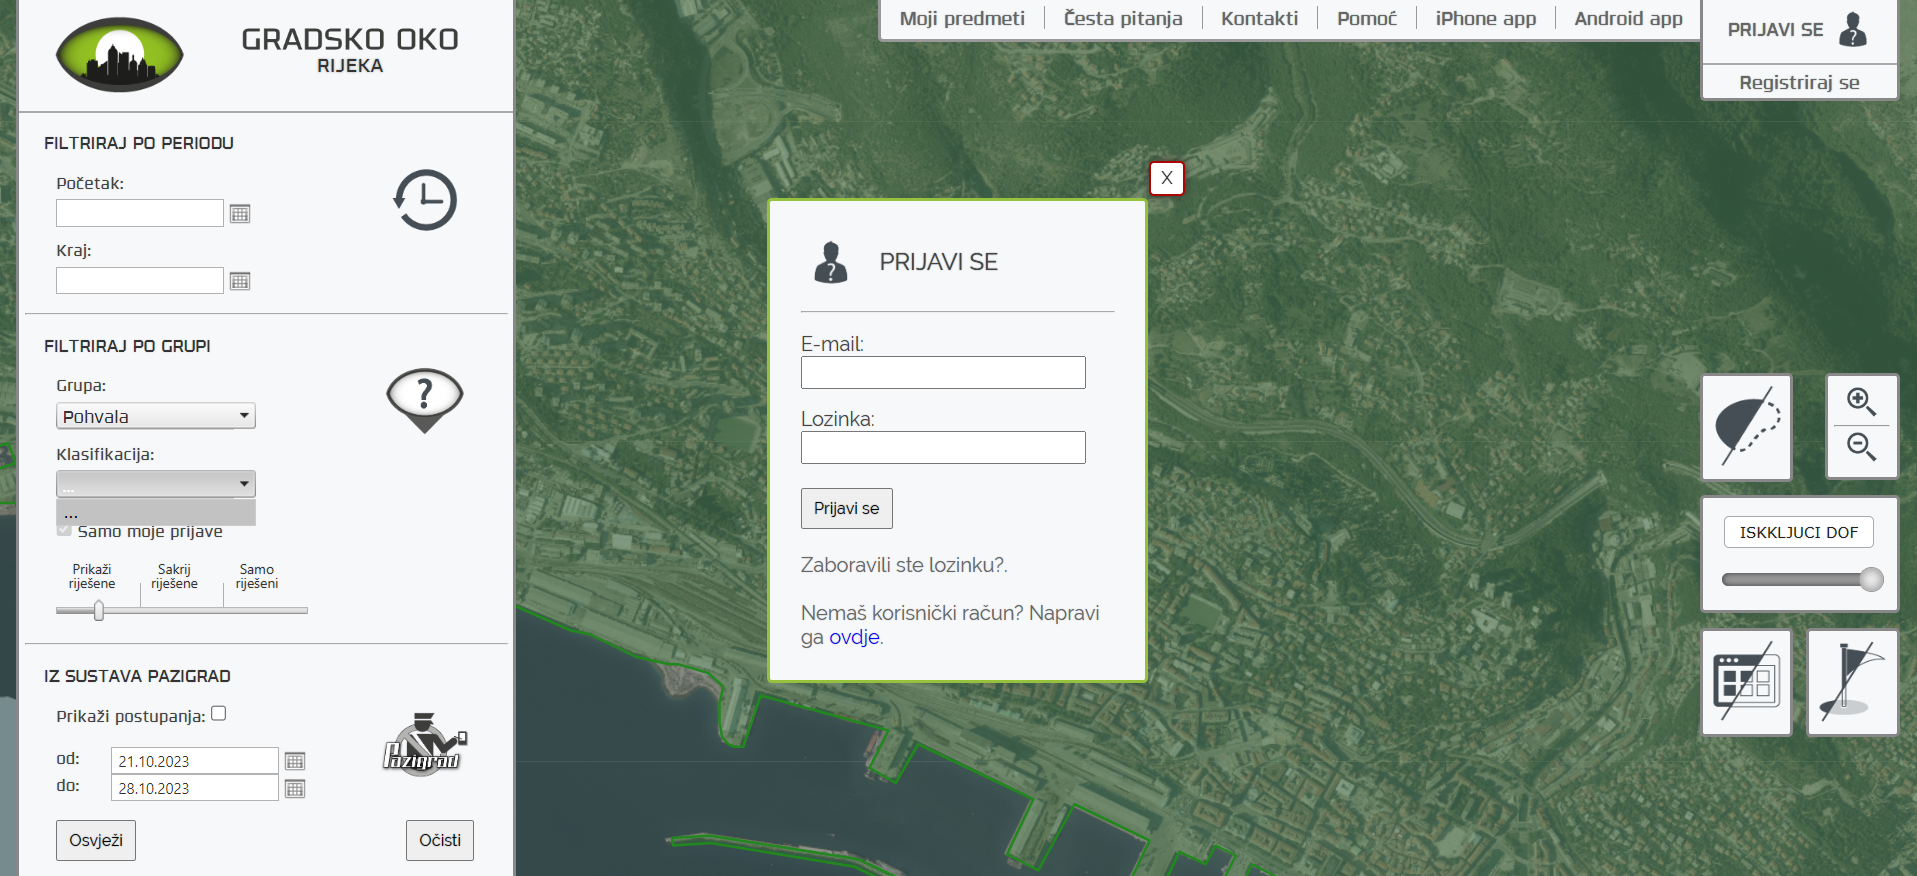
\includegraphics[width=\textwidth]{slike/GradskoOko.PNG}
			\caption{Aplikacija \textit{Gradsko oko} Grada Rijeke}
			\label{fig:gradskooko} %label mora biti drugaciji za svaku sliku
		\end{figure}
		
		\eject
		
		\section{Mogućnosti nadogradnje i skaliranja rješenja} 
		
		Uz male preinake moguće je prilagoditi aplikaciju da pruža istu potporu građanima nekog drugog grada ili općine, bilo u Hrvatskoj ili nekoj drugoj zemlji. Aplikacija bi se mogla skalirati i na veće jedinice lokalne samouprave kao što su županije, s obzirom da obično imaju sličan ustroj ureda i slične nadležnosti kao i gradovi. Ako se ideja skalira još više, aplikacija bi mogla pružati uslugu korisnicima cijele regije (npr. Slavonija, Dalmacija, Središnja Hrvatska) ili čak čitave države. U tom slučaju u aplikaciji bi bilo potrebno dodati mogućnost prepoznavanja nadležne jedinice lokalne samouprave prije predlaganja nadležnog ureda za konkretan problem. Takvo ponašanje bi se moglo implementirati uz malo prerađivanja i korištenje već postojećih funkcionalnosti aplikacije. Generalno gledano, aplikacija bi se mogla skalirati tako da pruža uslugu korisnicima nadnacionalnoj razini, primjerice na području cijele Europske Unije. Ponašanje aplikacije bi zapravo bilo isto uz potrebe skaliranja funkcionalnosti prepoznavanja nadležnih administrativnih jedinica na nadnacionalnoj razini. U tom slučaju aplikacija svakako mora pružati mogućnost prikaza na jeziku svake države u kojoj pruža uslugu. Glavna prepreka u ovakvoj implementaciji bi bila potreba za značajnijom infrastrukturalnom podrškom, prvenstveno u obliku velikih poslužitelja koji mogu obrađivati puno zahtjeva i pohranjivati velike količine podataka. Također, aplikacija bi na toj razini zahtjevala dobru suranju i koordinaciju velikog broja institucija u više različitih država što može biti zahtjevno.
		
		\eject
		
	\chapter{Specifikacija programske potpore}
		
	\section{Funkcionalni zahtjevi}
			
			\textbf{Nabrojeni funkcionalni zahtjevi:}
			\begin{packed_item}
				\item F01: registracija novog korisnika
				\item F02: prijava korisnika
				\item F03: podnošenje prijave oštećenja (naslov, opis, lokacija, slika - opcionalno, kategorija)
				\item F04: automatsko prepoznavanje kategorije prijave
				\item F05: mogućnost automatskog predlaganja nadovezivanja prijave na postojeću
				\item F06: pregledavanje podataka o korisničkom računu prijavljenog korisnika
				\item F07: uređivanje podataka o korisničkom računu prijavljenog korisnika
				\item F08: pregledavanje prijava prijavljenog korisnika
				\item F09: pregledavanje svih aktivnih prijava u sustavu preko interaktivne karte
				\item F10: mogućnost filtriranja prijava u sustavu prilikom pregledavanja
				\item F11: pregled statistike prijava
				\item F12: filtriranje statistike prijava
				\item F13: djelatnik gradskog ureda može odbaciti nevažeću prijavu
				\item F14: djelatnik gradskog ureda može proslijediti prijavu drugom uredu
				\item F15: djelatnik gradskog ureda može mijenjati status prijave
				\item F16: djelatnik gradskog ureda može objediniti prijave istog oštećenja
				\item F17: povratna informacija korisniku (ako je registriran) za svaku promjenu nad prijavom
				\item F18: pregled prijava ureda za djelatnike gradskog ureda
				\item F19: dodatno filtriranje prijava za djelatnike gradskog ureda
				\item F20: odjava iz sustava
				\item F21: brisanje korisničkog računa
			\end{packed_item}
			\eject
			
			\noindent \textbf{Dionici:}
			
			\begin{packed_enum}
				\item Gradska uprava
				\item Djelatnici gradskih ureda		
				\item Gradske službe
				\item Građani
				\item[] \begin{packed_item}
					\item Registrirani korisnici
					\item Neregistrirani korisnici
				\end{packed_item}
				\item Razvojni tim
			\end{packed_enum}
			
			
			\noindent \textbf{Aktori i njihovi funkcionalni zahtjevi:}
			
			\begin{packed_enum}
				
				\item  \underbar{Neregistrirani korisnik (inicijator) može:}
				\begin{packed_enum}
					\item napraviti svoj profil za koji mu je potrebno ime, prezime, email adresa i lozinka
					\item podnositi anonimnu prijavu koja sadrži naslov, opis, lokaciju i kategoriju oštećenja, a opcionalno i fotografiju i prijavu na koju se nadovezuje
					\item pregledavati postojeće prijave preko karte te ih filtrirati po vremenu i kategoriji oštećenja
					\item pregledavati statistiku postojećih prijava za odabran period, kategoriju oštećenja i prostor			
				\end{packed_enum}
								
				\item  \underbar{Registrirani korisnik (inicijator) može:}				
				\begin{packed_enum}					
					\item pregledavati i mijenjati osobne podatke
					\item obrisati svoj profil
					\item pregledavati svoje prijave
					\item podnositi prijavu koja sadrži naslov, opis, lokaciju i kategoriju oštećenja, a opcionalno i fotografiju i prijavu na koju se nadovezuje
					\item  pregledavati postojeće prijave preko karte te ih filtrirati po vremenu i kategoriji oštećenja
					\item pregledavati statistiku postojećih prijava za odabran period, kategoriju oštećenja i prostor
				\end{packed_enum}
				
				\item  \underbar{Djelatnik gradskog ureda (inicijator) može:}
				\begin{packed_enum}
					\item pregledavati prijave pristigle u njihov ured
					\item dodatno filtrirati prijave prilikom pregleda prema njihovom statusu
					\item mijenjati status prijavama
					\item objediniti prijave ako se referiraju na isti problem
					\item proslijediti prijave drugom uredu promjenom kategorije prijave
					\item označiti prijavu kao nevažeću
					\item pregledavati statistiku prijava
					\item dodatno filtrirati za koje prijave želi pregledati statistiku
				\end{packed_enum}
				
				\item  \underbar{Baza podataka (sudionik) može:}
				\begin{packed_enum}
					\item spremati sve podatke o korisnicima
					\item spremati sve podatke o gradskim uredima
					\item spremati sve podatke o prijavama
				\end{packed_enum}
				
			\end{packed_enum}
						
			\eject 
			
			\subsection{Obrasci uporabe}

					\noindent \underbar{\textbf{UC1 - Prijava oštećenja}}
					\begin{packed_item}
	
						\item \textbf{Glavni sudionik:} Korisnik
						\item  \textbf{Cilj:} Prijaviti oštećenje nadležnom gradskom uredu
						\item  \textbf{Sudionici:} Gradski ured, Baza podataka
						\item  \textbf{Preduvjet:} Korisnik je pronašao oštećenje koje želi prijaviti
						
						\item  \textbf{Opis osnovnog tijeka:}
						\item[] \begin{packed_enum}
							\item Korisnik odabire opciju za prijavljivanje oštećenja
							\item Korisnik popunjava podatke za prijavu oštećenja i podnosi prijavu
							\item Prijava se sprema u bazu podataka
							\item Korisnik dobiva jedinstveni kod svoje prijave.
						\end{packed_enum}
						
						\item  \textbf{Opis mogućih odstupanja:}
						\item[] \begin{packed_item}
							\item[2.a] Korisnik nije unio sve obavezne podatke u prijavu.
							\item[] \begin{packed_enum}
								\item Korisnik dobiva obavijest.
								\item Korisnik popunjava preostala obavezna polja ili odustaje od podnošenja prijave
							\end{packed_enum}
							
						\end{packed_item}
					\end{packed_item}
					
					
					\noindent \underbar{\textbf{UC2 - Pregled svih prijava}}
					\begin{packed_item}
						
						\item \textbf{Glavni sudionik:} Korisnik
						\item  \textbf{Cilj:} Pregled aktivnih prijava u sustavu
						\item  \textbf{Sudionici:} Baza podataka
						\item  \textbf{Preduvjet:} -
						
						\item  \textbf{Opis osnovnog tijeka:}
						\item[] \begin{packed_enum}
							\item Korisnik odabire glavnu stranicu
							\item Aplikacija prikazuje prijave na karti
							\item Korisnik odabire prijavu
							\item Prikazuju se podaci o prijavi
						\end{packed_enum}
					\end{packed_item}
				
				
				\noindent \underbar{\textbf{UC3 - Filtriranje prijava}}
				\begin{packed_item}
					
					\item \textbf{Glavni sudionik:} Korisnik
					\item  \textbf{Cilj:} Filtriranje prijava prilikom pregleda
					\item  \textbf{Sudionici:} Baza podataka
					\item  \textbf{Preduvjet:} Korisnik pregledava prijave na glavnoj stranici
					
					\item  \textbf{Opis osnovnog tijeka:}
					\item[] \begin{packed_enum}
						\item Korisnik odabire opciju filtriranja
						\item Korisnik odabire opcije kod filtriranja
						\item Aplikacija prikazuje filtrirane prijave
					\end{packed_enum}
				\end{packed_item}
				
				
				\noindent \underbar{\textbf{UC4 - Pregled statistike prijava}}
				\begin{packed_item}
					
					\item \textbf{Glavni sudionik:} Korisnik ili Djelatnik gradskog ureda
					\item  \textbf{Cilj:} Pregled statistike prijava u sustavu
					\item  \textbf{Sudionici:} Baza podataka
					\item  \textbf{Preduvjet:} -
					
					\item  \textbf{Opis osnovnog tijeka:}
					\item[] \begin{packed_enum}
						\item Korisnik odabire opciju za pregledavanje statistike prijava
						\item Aplikacija prikazuje razne podatke za prijave u sustavu
					\end{packed_enum}
				\end{packed_item}
				
				
				\noindent \underbar{\textbf{UC5 - Filtriranje statistike prijava}}
				\begin{packed_item}
					
					\item \textbf{Glavni sudionik:} Korisnik ili Djelatnik Gradskog ureda
					\item  \textbf{Cilj:} Filtriranje prijava prilikom pregleda statistike
					\item  \textbf{Sudionici:} Baza podataka
					\item  \textbf{Preduvjet:} Korisnik je odabrao opciju pregleda statistike prijava
					
					\item  \textbf{Opis osnovnog tijeka:}
					\item[] \begin{packed_enum}
						\item Korisnik odabire opcije za filtriranje
						\item Aplikacija prikazuje statistiku za filtrirane prijave
					\end{packed_enum}
				\end{packed_item}
				
				
				\noindent \underbar{\textbf{UC6 - Registracija}}
				\begin{packed_item}
					
					\item \textbf{Glavni sudionik:} Neregistrirani korisnik ili Djelatnik gradskog ureda
					\item  \textbf{Cilj:} Izrada korisničkog računa za korisnika ili novi gradski ured
					\item  \textbf{Sudionici:} Baza podataka
					\item  \textbf{Preduvjet:} -
					
					\item  \textbf{Opis osnovnog tijeka:}
					\item[] \begin{packed_enum}
						\item Korisnik odabire opciju registracije
						\item Korisnik popunjava podatke za izradu korisničkog računa i potvrđuje registraciju
						\item Podaci o novom računu se spremaju u bazu podataka
					\end{packed_enum}
					
					\item  \textbf{Opis mogućih odstupanja:}
					\item[] \begin{packed_item}
						\item[2.a] Unesena email adresa je već zauzeta
						\item[] \begin{packed_enum}
							\item Aplikacija prikazuje prikladnu obavijest i vraća korisnika na stranicu za registraciju
							\item Korisnik unosi drugu email adresu ili odustaje od registracije
						\end{packed_enum}
						\item[2.b] Unesena lozinka je preduga ili prekratka
						\item[] \begin{packed_enum}
							\item Aplikacija prikazuje prikladnu obavijest i vraća korisnika na stranicu za registraciju
							\item Korisnik unosi drugu lozinku ili odustaje od registracije
						\end{packed_enum}
					\end{packed_item}
				\end{packed_item}
				
				
				\noindent \underbar{\textbf{UC7 - Pregled vlastitih prijava}}
				\begin{packed_item}
					
					\item \textbf{Glavni sudionik:} Registrirani korisnik
					\item  \textbf{Cilj:} Pregled prijava koje je korisnik do sada podnio
					\item  \textbf{Sudionici:} Baza podataka
					\item  \textbf{Preduvjet:} Korisnik pregledava svoj korisnički račun
					
					\item  \textbf{Opis osnovnog tijeka:}
					\item[] \begin{packed_enum}
						\item Registrirani korisnik prilikom pregleda korisničkog računa odlazi na sekciju pregleda vlastitih prijava
						\item Aplikacija prikazuje listu dosadašnjih prijava Registriranog korisnika
						\item Registrirani korisnik odabire prijavu
						\item Prikazuju se podaci o prijavi
					\end{packed_enum}
					
					\item  \textbf{Opis mogućih odstupanja:}
					\item[] \begin{packed_item}						
						\item[3.a] Registrirani korisnik ne želi pregledati konkretnu prijavu
						\item[] \begin{packed_enum}
							\item Korisnik nakon pregleda liste prijava izlazi iz opcije pregleda vlastitih prijava
						\end{packed_enum}
					\end{packed_item}
				\end{packed_item}
				
				
				\noindent \underbar{\textbf{UC8 - Pregled korisničkog računa}}
				\begin{packed_item}
					
					\item \textbf{Glavni sudionik:} Registrirani korisnik
					\item  \textbf{Cilj:} Pregled vlastitog korisničkog računa
					\item  \textbf{Sudionici:} Baza podataka
					\item  \textbf{Preduvjet:} -
					
					\item  \textbf{Opis osnovnog tijeka:}
					\item[] \begin{packed_enum}
						\item Registrirani korisnik odabire prikaz stranice svojeg profila
						\item Aplikacija prikazuje podatke o korisničkom računu
						\item Registrirani korisnik pregledava podatke o svojem korisničkom računu
					\end{packed_enum}
				\end{packed_item}
				
				
				\noindent \underbar{\textbf{UC9 - Promjena podataka o računu}}
				\begin{packed_item}
					
					\item \textbf{Glavni sudionik:} Registrirani korisnik
					\item  \textbf{Cilj:} Promjena podataka o korisničkom računu
					\item  \textbf{Sudionici:} Baza podataka
					\item  \textbf{Preduvjet:} Registrirani korisnik pregledava svoj korisnički račun
					
					\item  \textbf{Opis osnovnog tijeka:}
					\item[] \begin{packed_enum}
						\item Registrirani korisnik mijenja željene podatke o računu
						\item Registrirani korisnik potvrđuje izmjene i vraća se u pregled korisničkog računa
						\item Izmijenjeni podaci se spremaju u bazu podataka
					\end{packed_enum}
					
					\item  \textbf{Opis mogućih odstupanja:}
					\item[] \begin{packed_item}
						\item[4.a] Registrirani korisnik je promijenio email adresu u već zauzetu email adresu
						\item[] \begin{packed_enum}
							\item Aplikacija javlja pogrešku s odgovarajućom porukom i vraća korisnika na stranicu za registraciju
							\item Registrirani korisnik unosi drugu email adresu ili odustaje od promjene email adrese ili uređivanja podataka o korisničkom računu
						\end{packed_enum}
					\end{packed_item}
				\end{packed_item}
				
				
				\noindent \underbar{\textbf{UC10 - Brisanje korisničkog računa}}
				\begin{packed_item}
					
					\item \textbf{Glavni sudionik:} Registrirani korisnik
					\item  \textbf{Cilj:} Brisanje korisničkog računa
					\item  \textbf{Sudionici:} Baza podataka
					\item  \textbf{Preduvjet:} Registrirani korisnik pregledava svoj korisnički račun
					
					\item  \textbf{Opis osnovnog tijeka:}
					\item[] \begin{packed_enum}
						\item Registrirani korisnik odlazi na stranicu svojeg profila
						\item Registrirani korisnik prilikom pregledavanja svojeg korisničkog računa odabire opciju brisanja korisničkog računa
						\item Korisnički račun se briše, korisnik postaje Neregistrirani korisnik i aplikacija ga vraća na početnu stranicu
					\end{packed_enum}
				\end{packed_item}
				
				
				\noindent \underbar{\textbf{UC11 - Prijava u sustav}}
				\begin{packed_item}
					
					\item \textbf{Glavni sudionik:} Registrirani korisnik ili Djelatnik gradskog ureda
					\item  \textbf{Cilj:} Prijava korisnika u sustav
					\item  \textbf{Sudionici:} Baza podataka
					\item  \textbf{Preduvjet:} -
					
					\item  \textbf{Opis osnovnog tijeka:}
					\item[] \begin{packed_enum}
						\item Korisnik odabire opciju prijave
						\item Korisnik unosi svoju email adresu i lozinku
						\item Aplikacija otvara početnu stranicu
					\end{packed_enum}
					
					\item  \textbf{Opis mogućih odstupanja:}
					\item[] \begin{packed_item}
						\item[2.a] Registrirani korisnik unosi nevažeću kombinaciju email adrese i lozinke
						\item[] \begin{packed_enum}
							\item Aplikacija javlja pogrešku s odgovarajućom porukom i traži ponovnu prijavu
							\item Korisnik unosi ispravnu kombinaciju ili odustaje od prijave i koristi aplikaciju u anonimnom načinu
						\end{packed_enum}
					\end{packed_item}
				\end{packed_item}
				
				
				\noindent \underbar{\textbf{UC12 - Odjava iz sustava}}
				\begin{packed_item}
					
					\item \textbf{Glavni sudionik:} Registrirani korisnik ili Djelatnik gradskog ureda
					\item  \textbf{Cilj:} Odjava korisnika iz sustav
					\item  \textbf{Sudionici:} -
					\item  \textbf{Preduvjet:} Korisnik je prijavljen u sustav
					
					\item  \textbf{Opis osnovnog tijeka:}
					\item[] \begin{packed_enum}
						\item korisnik odabire ikonu svojeg profila
						\item Korisnik na ponuđenom izborniku odabire opciju odjave iz sustava
						\item Aplikacija otvara početnu stranicu u anonimnom načinu
					\end{packed_enum}
				\end{packed_item}
				
				
				\noindent \underbar{\textbf{UC13 - Obrada prijava}}
				\begin{packed_item}
					
					\item \textbf{Glavni sudionik:} Djelatnik gradskog ureda
					\item  \textbf{Cilj:} Obrada prijave u gradskom uredu
					\item  \textbf{Sudionici:} Baza podataka, Gradska služba
					\item  \textbf{Preduvjet:} Djelatnik pregledava prijave ureda
					
					\item  \textbf{Opis osnovnog tijeka:}
					\item[] \begin{packed_enum}
						\item Djelatnik gradskog ureda odabire prijavu
						\item Djelatnik mijenja status prijave
						\item Prijava se delegira nadležnoj gradskoj službi ako joj je status promijenjen u \textit{u procesu}
					\end{packed_enum}
				\end{packed_item}
				
				
				\noindent \underbar{\textbf{UC14 - Odbacivanje pristigle prijave}}
				\begin{packed_item}
					
					\item \textbf{Glavni sudionik:} Djelatnik gradskog ureda
					\item  \textbf{Cilj:} Odbacivanje nevaljale prijave
					\item  \textbf{Sudionici:} Baza podataka
					\item  \textbf{Preduvjet:} Djelatnik gradskog ureda obrađuje prijavu
					
					\item  \textbf{Opis osnovnog tijeka:}
					\item[] \begin{packed_enum}
						\item Djelatnik procjenjuje da prijava nije utemeljena
						\item Djelatnik odabire opciju za odbacivanje prijave
					\end{packed_enum}
				\end{packed_item}
				
				
				\noindent \underbar{\textbf{UC15 - Prebacivanje prijave na drugi ured}}
				\begin{packed_item}
					
					\item \textbf{Glavni sudionik:} Djelatnik gradskog ureda
					\item  \textbf{Cilj:} Prosljeđivanje prijave nadležnom gradskom uredu
					\item  \textbf{Sudionici:} Baza podataka
					\item  \textbf{Preduvjet:} Djelatnik gradskog ureda obrađuje prijavu
					
					\item  \textbf{Opis osnovnog tijeka:}
					\item[] \begin{packed_enum}
						\item Djelatnik procjenjuje da je neki drugi ured nadležan za ovu prijavu
						\item Djelatnik odabire opciju prebacivanja prijave na drugi ured
						\item Djelatnik odabire novu kategoriju te prijave (čime indirektno mijenja ured) i potvrđuje unos
					\end{packed_enum}
				\end{packed_item}
				
				
				\noindent \underbar{\textbf{UC16 - Objedinjenje nepovezanih prijava}}
				\begin{packed_item}
					
					\item \textbf{Glavni sudionik:} Djelatnik gradskog ureda
					\item  \textbf{Cilj:} Objedinjavanje prijava istog oštećenja
					\item  \textbf{Sudionici:} Baza podataka
					\item  \textbf{Preduvjet:} Djelatnik gradskog ureda obrađuje prijavu
					
					\item  \textbf{Opis osnovnog tijeka:}
					\item[] \begin{packed_enum}
						\item Djelatnik procjenjuje da postoji više prijava istog oštećenja
						\item Djelatnik odabire opciju objedinjavanja prijava
						\item Djelatnik odabire prijave koje želi objediniti i potvrđuje odabir
					\end{packed_enum}
				\end{packed_item}
				
				
				\noindent \underbar{\textbf{UC17 - Slanje povratnih informacija}}
				\begin{packed_item}
					
					\item \textbf{Glavni sudionik:} Djelatnik gradskog ureda
					\item  \textbf{Cilj:} Informiranje prijavitelja o promjenama u njegovoj prijavi
					\item  \textbf{Sudionici:} Baza podataka
					\item  \textbf{Preduvjet:} Djelatnik gradskog ureda je prilikom obrade prijave izvršio neku radnju/promjenu nad prijavom
					
					\item  \textbf{Opis osnovnog tijeka:}
					\item[] \begin{packed_enum}
						\item Aplikacija šalje obavijest prijavitelju o promjenama vezanim uz prijavu
					\end{packed_enum}
					
					\item  \textbf{Opis mogućih odstupanja:}
					\item[] \begin{packed_item}
						\item[1.a] Prijava je anonimna
						\item[] \begin{packed_enum}
							\item Aplikacija ne radi ništa
						\end{packed_enum}
					\end{packed_item}
				\end{packed_item}
				
				
				\noindent \underbar{\textbf{UC18 - Pregled prijava gradskog ureda}}
				\begin{packed_item}
					
					\item \textbf{Glavni sudionik:} Djelatnik gradskog ureda
					\item  \textbf{Cilj:} Pregledavanje prijava koje gradski ured obrađuje/treba obraditi/je obradio
					\item  \textbf{Sudionici:} Baza podataka
					\item  \textbf{Preduvjet:} -
					
					\item  \textbf{Opis osnovnog tijeka:}
					\item[] \begin{packed_enum}
						\item Djelatnik gradskog ureda odlazi na glavnu stranicu za Djelatnike gradskog ureda
						\item Aplikacija prikazuje prijave iz liste novopristiglih prijava
					\end{packed_enum}
				\end{packed_item}
				
				
				\noindent \underbar{\textbf{UC19 - Filtriranje prijava gradskog ureda}}
				\begin{packed_item}
					
					\item \textbf{Glavni sudionik:} Djelatnik gradskog ureda
					\item  \textbf{Cilj:} Filtriranje prijava koje gradski ured mora obraditi/obrađuje/je obradio
					\item  \textbf{Sudionici:} Baza podataka
					\item  \textbf{Preduvjet:} Djelatnik gradskog ureda pregledava prijave
					
					\item  \textbf{Opis osnovnog tijeka:}
					\item[] \begin{packed_enum}
						\item Djelatnik gradskog ureda odabire listu prijava prema statusu prijava
						\item Aplikacija prikazuje odabranu listu prijava
					\end{packed_enum}
				\end{packed_item}
				
				
				\noindent \underbar{\textbf{UC20 - Prepoznavanje kategorije}}
				\begin{packed_item}
					
					\item \textbf{Glavni sudionik:} Korisnik
					\item  \textbf{Cilj:} Automatsko prepoznavanje kategorije oštećenja
					\item  \textbf{Sudionici:} Baza podataka
					\item  \textbf{Preduvjet:} Korisnik podnosi prijavu oštećenja
					
					\item  \textbf{Opis osnovnog tijeka:}
					\item[] \begin{packed_enum}
						\item Aplikacija dohvaća popis ključnih riječi i njihovih kategorija
						\item Korisnik unosi opis oštećenja
						\item Aplikacija na temelju prepoznanih ključnih riječi predlaže kategoriju
						\item Korisnik ostavlja predloženu kategoriju ili ručno odabire ispravnu kategoriju
					\end{packed_enum}
				\end{packed_item}
				
				
				\noindent \underbar{\textbf{UC21 - Nadovezivanje prijave}}
				\begin{packed_item}
					
					\item \textbf{Glavni sudionik:} Korisnik
					\item  \textbf{Cilj:} Nadovezivanje prijave na već postojeću prijavu istog oštećenja
					\item  \textbf{Sudionici:} Baza podataka
					\item  \textbf{Preduvjet:} Korisnik podnosi prijavu oštećenja
					
					\item  \textbf{Opis osnovnog tijeka:}
					\item[] \begin{packed_enum}
						\item Korisnik potvrđuje i podnosi prijavu
						\item Aplikacija provjerava ako u bazi podataka već postoji slična prijava
						\item Ako takva postoji, aplikacija nudi korisniku da se nadoveže na već postojeću prijavu
						\item Korisnik može nadovezati prijavu ili ju podnijeti kao samostalnu
					\end{packed_enum}
				\end{packed_item}
				
				\eject
					
				\subsubsection{Dijagrami obrazaca uporabe}
					
					\begin{figure}[H]
						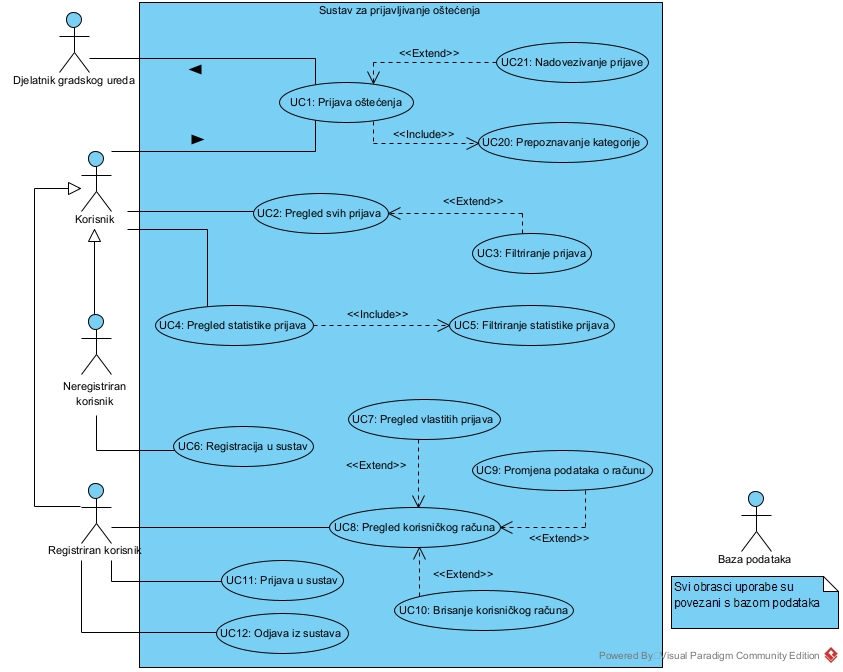
\includegraphics[width=\textwidth]{slike/Funkcionalnosti_korisnikaUCD.jpg} %veličina u odnosu na širinu linije
						\caption{Dijagram obrasca uporabe, mogućnosti korisnika}
						\label{fig:dijagramObrascaUporabe1} %label mora biti drugaciji za svaku sliku
					\end{figure}
					
					\begin{figure}[H]
						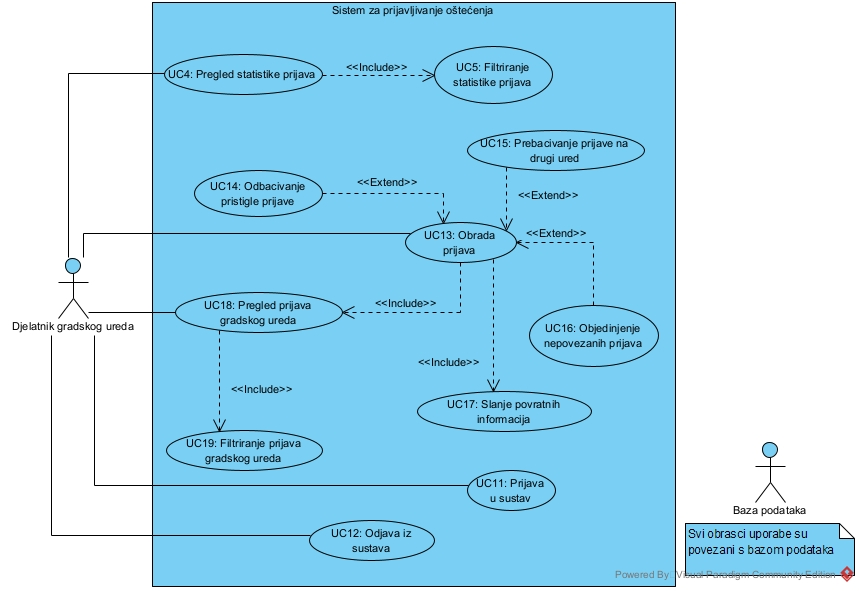
\includegraphics[width=\textwidth]{slike/Obrada_prijavaUCD.jpg} %veličina u odnosu na širinu linije
						\caption{Dijagram obrasca uporabe, obrada prijava}
						\label{fig:dijagramObrascaUporabe2} %label mora biti drugaciji za svaku sliku
					\end{figure}
					
				\eject		
				
			\subsection{Sekvencijski dijagrami}
				
				\textbf{Obrasci uporabe - UC06, UC11 - Registracija u sustav, Prijava u sustav}
				
				Korisnik(može biti i djelatnik) na naslovnoj stranici odabire opciju prijave ili registracije te mu se zatim otvara prikladna stranica. Ako se radi o stranici za prijavu, korisnik unosi svoj email i zaporku i potvrđuje unos. Ako su uneseni podaci validni korisniku se prikazuje naslovna stranica za prijavljenog korisnika, odnosno za djelatnika gradskog ureda. U suprotnom se korisnika obavještava o grešci i ponovno traži unos podataka za prijavu. Ako se radi o stranici za registraciju, korisnik mora unijeti svoje ime, prezime, datum rođenja, email adresu i lozinku. Ako se registrira novi gradski ured, potrebno je označiti tu opciju. U tom slučaju se traži unos imena ureda, email adresa, lozinka i barem jedna kategorija za koju će novi gradski ured biti nadležan. Sustav provjerava u bazi ako za danu email adresu već postoji korisnički račun. Ako račun već postoji, sustav korisniku javlja grešku i ponovno traži unos podataka za registraciju. Ako je unos dobar, korisniku se prikazuje naslovna stranica za prijavljenog korisnika, odnosno za djelatnika gradskog ureda. Korisnik ne mora odabrati opciju prijave ili registracije. U tom slučaju koristi stranicu kao anoniman neregistrirani korisnik. Djelatnik se mora prijaviti ili registrirati ured da bi obavljao svoju funkcionalnost.
				
				\begin{figure}[H]
					\includegraphics[width=\textwidth]{slike/Prijava_registracijaSD.jpg} %veličina u odnosu na širinu linije
					\caption{Sekvencijski dijagram, prijava/registracija}
					\label{fig:sekvencijskiDijagram1} %label mora biti drugaciji za svaku sliku
				\end{figure}
				\eject
				
				\textbf{Obrasci uporabe - UC1 - Prijava oštećenja}
				
				Korisnik odabire opciju podnošenja nove prijave oštećenja. U prijavi korisnik upisuje kratak naslov, opis oštećenja, lokaciju i kategoriju. Korisnik također može priložiti fotografiju oštećenja. Lokaciju korisnik može priložiti preko interaktivne karte, upisom adrese ili se lokacija može izvući iz meta podataka fotografija, ako je fotografija priložena. Aplikacija će sama pokušati prepoznati kategoriju oštećenja i na temelju toga i ponuditi nadležan ured. Za to su joj potrebne ključne riječi za svaku kategoriju koje je aplikacija dohvatila prilikom odabira podnošenja nove prijave. Aplikacija nakon unosa podataka dohvaća postojeće prijave koje imaju sličnu lokaciju, istu kategoriju i koje još nisu obrađene. Ako takve prijave postoje, aplikacija će korisniku ponuditi da svoju prijavu nadoveže na jednu od ponuđenih prijava. Korisnik može, ali i ne mora nadovezati svoju prijavu kada mu je ta opcija ponuđena. Nakon podnošenja prijave korisnik dobiva kod prijave preko koje može pratiti njezino stanje.
				
				\begin{figure}[H]
					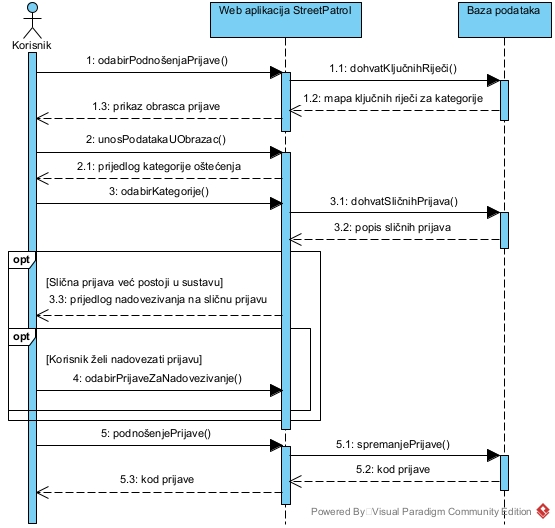
\includegraphics[width=\textwidth]{slike/Podnosenje_prijaveSD.jpg} %veličina u odnosu na širinu linije
					\caption{Sekvencijski dijagram, podnošenje prijave}
					\label{fig:sekvencijskiDijagram2} %label mora biti drugaciji za svaku sliku
				\end{figure}
				\eject
				
				\textbf{Obrasci uporabe - UC13, UC14, UC15, UC16, UC17, UC18, UC19 - Obrada prijava, Odbacivanje pristigle prijave, Prebacivanje prijave na drugi ured, Objedinjenje nepovezanih prijava, Slanje povratnih informacija, Pregled prijava gradskog ureda, filtriranje prijava gradskog ureda}
				
				Djelatnik gradskog ureda odabire jednu od 3 lista prijava, jedna za svaki status. Za izlistane prijave djelatniku se prikazuju podaci o svakoj prijavi. Djelatnik dalje može promijeniti status prijave. Ako vidi da je oštećenje u toj prijavu već prijavljeno, djelatnik može odabrati sve takve prijave i objediniti ih. Ako utvrdi da njegov ured nije nadležan za ovu prijavu, djelatnik odabire novu kategoriju i time prosljeđuje prijavu drugom uredu. Ako je prijava u potpunosti nevaljana djelatnik ju može odbaciti. Bilo koja od ovih radnji nad prijavom rezultirat će slanjem povratne informacije korisniku koji je podnio prijavu, ako je taj korisnik registriran.
				
				\begin{figure}[H]
					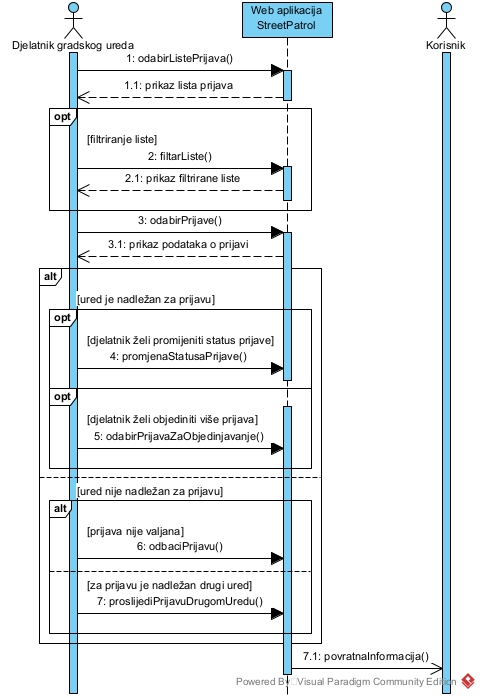
\includegraphics[width=\textwidth]{slike/Obrada_prijavaSD.jpg} %veličina u odnosu na širinu linije
					\caption{Sekvencijski dijagram, obrada prijava}
					\label{fig:sekvencijskiDijagram3} %label mora biti drugaciji za svaku sliku
				\end{figure}
				\eject


	
		\section{Ostali zahtjevi}
			
			\begin{packed_item}
				\item Sustav treba podržati rad više korisnika u stvarnom vremenu
				\item Sustav treba biti implementiran kao web aplikacija s responzivnim dizajnom
				\item Aplikacija mora koristiti HTTPS protokol
				\item Aplikacija mora biti jednostavna za korištenje
				\item Neispravno korištenje korisničkog sučelja ne smije narušiti cjelokupan rad sustava
				\item Izvršavanje bilo koje akcije na aplikaciji ne smije trajati dulje od 10 sekundi
				\item Osjetljivi podaci, kao što su lozinke korisnika, se u bazu podataka moraju spremati u kriptiranom obliku koristeći \textit{bcrypt} algoritam
			\end{packed_item}
			
	\chapter{Arhitektura i dizajn sustava}
		
		Arhitektura ovog sustava je bazirana na arhitekturi klijent-poslužitelj. Sustav se sastoji od 3 sloja: sloj korisničkog sučelja, sloj aplikacijske logike, sloj podataka.
		
		\textbf{Web preglednik} je program preko kojeg korisnik koristi aplikaciju. Preglednik omogućuje klijentu komunikaciju s web poslužiteljem aplikacije. Preglednik nam omogućava prikaz sloja korisničkog sučelja sustava. Korisnik preko web preglednika komunicira s web poslužiteljem slanjem i primanjem HTTP zahtjeva. Primljene podatke i datoteke web preglednik zna interpretirati i prikazati korisniku tako da sama interakcija s aplikacijom bude jednostavna. Neki od popularnih web preglednika su Chrome, Safari i Edge.
		
		\textbf{Web poslužitelj} je računalo na kojem se aplikacija pokreće. Na njemu se dakle nalazi sloj aplikacijske logike. Web poslužitelj aplikaciji prosljeđuje zahtjeve na obradu i njezine odgovore prosljeđuje natrag klijentima. Web aplikacija na poslužitelju obrađuje zaprimljene zahtjeve. Ako obrada zahtjeva to zahtjeva, web aplikacija dodatno komunicira sa slojem podataka.
		
		\textbf{Baza Podataka} predstavlja sloj podataka. U bazi podataka se na siguran način spremaju svi podaci koje je potrebno trajno čuvati. To podrazumijeva podatke o prijavama, korisničkim računima i slično. Takvi podaci moraju ostati očuvani i ako je rad aplikacije prekinut iz bilo kojeg razloga. Baza podataka je detaljnije opisana u poglavlju  \ref{sec:bazaPodataka}.
		
		\textbf{Web aplikacija} je podijeljena na frontend i backend.
		
		\textbf{Frontend} je zapravo prezentacijski dio aplikacije i zadužen je za interakciju s korisnikom. On oblikuje korisničko sučelje i samim time definira što će korisnik vidjeti na web pregledniku kada koristi aplikaciju.
		
		\textbf{Backend} je dio aplikacije koji obrađuje zahtjeve i kontrolira rad ostalih dijelova sustava. Baceknd je usko povezan s web poslužiteljem.
		
		Za izradu backend dijela aplikacije odabrali smo programski jezik Java s radnim okvirom Spring Boot. Spring Boot radni okvir koristi višeslojnu arhitekturu u kojoj svaki sloj komunicira sa slojem koji se u hijerarhiji nalazi iznad ili ispod njega. Arhitektura Spring Boota se sastoji od četiri sloja:
		\begin{packed_item}
			\item \textbf{Prezentacijski sloj} (\textit{Presentation layer}) - Ovo je najviši sloj arhitekture i predstavlja frontend dio aplikacije. Ovaj sloj prima HTTP zahtjeve i vrši autentifikaciju. Također vrši pretvorbu JSON objekata u objekte u Javi i obrnuto. Na kraju svoje obrade Prezentacijski sloj prosljeđuje HTTP zahtjev sljedećem sloju.
			
			\item \textbf{Poslovni sloj} (\textit{Business layer}) - Ovaj sloj sadrži svu poslovnu logiku te je zadužen za validaciju i autorizaciju.
			
			\item \textbf{Sloj postojanosti} (\textit{Persistence layer}) - Ovaj sloj sadrži logiku vezanu uz pohranu u bazu podataka. Sloj pretvara zapise iz baze podataka u objekte iz poslovnog sloja i obrnuto.
			
			\item \textbf{Sloj baze podataka} (\textit{Database layer}) - Ovaj sloj sadrži bazu podataka ili više njih. Sloj je zadužen za obavljanje CRUD (copy, read, update, delete) operacija.
		\end{packed_item}
		
		\begin{figure}[H]
			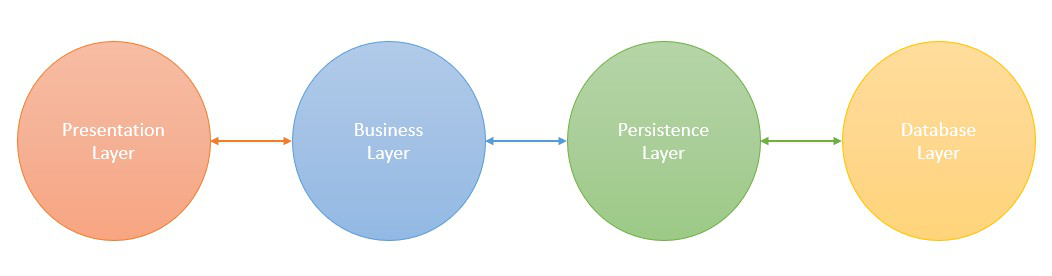
\includegraphics[width=\textwidth]{slike/slojeviArhitekture.jpg} %veličina u odnosu na širinu linije
			\caption{Prikaz Spring Boot arhitekture}
			\label{fig:SpringBootArh} %label mora biti drugaciji za svaku sliku
		\end{figure}
		
		Za razvoj frontend dijela aplikacije odlučili smo koristiti programski jezik JavaScript uz radni okvir React. React omogućuje jednostavnu izradu korisničkog sučelja preko JavaScripta, bez direktnog korištenja HTML-a.
		
		Za razvojne okoline smo odlučili koristiti IntelliJ IDEA za rad u Spring Boot radnom okviru i Visual Studio Code za rad u React radnom okviru.
		
	\eject
	
		\section{Baza podataka}
		\label{sec:bazaPodataka}
		
		Ovaj sustav će za svoje potrebe koristiti relacijsku bazu podataka implementirana u PostgreSQL-u. Ovakav tip baze podataka svojom strukturom omogućuje jednostavno modeliranje elemenata iz stvarnog svijeta i zbog toga je široko primjenjiv. Odabrali smo implementaciju u PostgreSQL-u jer smo s ovom implementacijom već dobro upoznati. Relacijske baze podataka se sastoje od relacija. Relacije su predstavljene tablicama koje su definirane svojim nazivom i skupom atributima. Bazu podataka koristimo za jednostavnu i sigurnu pohranu, izmjenu, umetanje i dohvat podataka potrebnih za rad sustava. Naša baza podataka se sastoji od sljedećih relacija, odnosno tablica:
		
		\begin{packed_item}
			\item Users
			\item Report
			\item Image
			\item Category
			\item CategoryKeywords
			\item ReportGroup 
			\item Feedback
			\item CityOffice
		\end{packed_item}
		
			\subsection{Opis tablica}
			
			\textbf{Users} tablica čuva podatke o korisničkim računima koje korisnici izrađuju tijekom registracije. Tablica je povezana vezom \textit{One-to-Many} s tablicom \textit{Report} preko atributa \textit{userID}.
			
			\begin{longtblr}[
					label=Users,
					entry=none
				]{
					width = \textwidth,
					colspec={|X[6,l]|X[6, l]|X[20, l]|}, 
					rowhead = 1,
				} %definicija širine tablice, širine stupaca, poravnanje i broja redaka naslova tablice
				\hline \SetCell[c=3]{c}{\textbf{Users}}	 \\ \hline[3pt]
				\SetCell{LightGreen} userID & INT & jedinstveni identifikator korisnika \\ \hline
				email & VARCHAR & email adresa korisnika \\ \hline 
				firstName & VARCHAR & ime korisnika \\ \hline
				lastName & VARCHAR & prezime korisnika \\ \hline 
				password & VARCHAR & kriptirana lozinka za korisnički račun \\ \hline 
			\end{longtblr}
			
			\textbf{Report} tablica čuva podatke o pojedinim prijavama oštećenja koje korisnici podnose. Tablica je povezana vezom \textit{Many-to-One} s tablicom \textit{Users} preko atributa \textit{userID}, \textit{Many-to-One} vezom s tablicom \textit{Category} preko atributa \textit{categoryID}. Također postoji auto-refleksivna \textit{Many-to-One} veza kojom se modelira nadovezivanje prijava.
			
			\begin{longtblr}[
				label=Report,
				entry=none
				]{
					width = \textwidth,
					colspec={|X[8,l]|X[6, l]|X[20, l]|}, 
					rowhead = 1,
				} %definicija širine tablice, širine stupaca, poravnanje i broja redaka naslova tablice
				\hline \SetCell[c=3]{c}{\textbf{Report}}	 \\ \hline[3pt]
				\SetCell{LightGreen} reportID & INT & jedinstveni identifikator prijave \\ \hline
				description & VARCHAR & opis oštećenja \\ \hline 
				reportTS & TIMESTAMP & vrijeme prijave \\ \hline 
				reportHeadline & VARCHAR & naslov prijave \\ \hline 
				lng & REAL & geografska dužina lokacije oštećenja \\ \hline
				lat & REAL & geografska širina lokacije oštećenja \\ \hline
				\SetCell{LightBlue} userID & INT & jedinstveni identifikator korisnika koji je podnio prijavu \\ \hline 
				\SetCell{LightBlue} categoryID & INT & jedinstveni identifikator kategorije oštećenja \\ \hline
				\SetCell{LightBlue} isConnectedToID & INT & jedinstveni identifikator prijave na koju je ova prijava nadovezana \\ \hline
			\end{longtblr}
			
			\textbf{Image} tablica čuva podatke o slikama koje se prilažu u prijavama oštećenja. Tablica je povezana \textit{Many-to-One} vezom s tablicom \textit{Report} preko atributa \textit{reportID}.
			
			\begin{longtblr}[
				label=Image,
				entry=none
				]{
					width = \textwidth,
					colspec={|X[6,l]|X[6, l]|X[20, l]|}, 
					rowhead = 1,
				} %definicija širine tablice, širine stupaca, poravnanje i broja redaka naslova tablice
				\hline \SetCell[c=3]{c}{\textbf{Image}}	 \\ \hline[3pt]
				\SetCell{LightGreen} imageID & INT & jedinstveni identifikator slike \\ \hline
				\SetCell{LightBlue} reportID & INT & jedinstveni identifikator prijave kojoj slika pripada \\ \hline
				URL & VARCHAR & URL slike \\ \hline 
			\end{longtblr}
			
			\textbf{Category} tablica čuva podatke o kategorijama kojima oštećenje može pripadati. Tablica je povezana \textit{One-to-Many} vezom s tablicom \textit{Report} preko atributa \textit{categoryID}, \textit{Many-to-One} vezom s tablicom \textit{CityOffice} preko atributa \textit{cityOfficeID} i \textit{One-to-Many} vezom s tablicom \textit{CategoryKeywords} preko atributa \textit{categoryID}.
			
			\begin{longtblr}[
				label=Category,
				entry=none
				]{
					width = \textwidth,
					colspec={|X[6,l]|X[6, l]|X[20, l]|}, 
					rowhead = 1,
				} %definicija širine tablice, širine stupaca, poravnanje i broja redaka naslova tablice
				\hline \SetCell[c=3]{c}{\textbf{Category}}	 \\ \hline[3pt]
				\SetCell{LightGreen} categoryID & INT & jedinstveni identifikator kategorije \\ \hline
				categoryName & VARCHAR & naziv kategorije \\ \hline 
				\SetCell{LightBlue} cityOfficeID & INT & jedinstveni identifikator gradskog ureda koji obrađuje prijave oštećenja iz ove kategorije \\ \hline
			\end{longtblr}

			\textbf{CategoryKeywords} tablica čuva podatke o ključnim riječima po kojima se može identificirati kategorija oštećenja. Tablica je povezana \textit{Many-to-One} vezom s tablicom \textit{Category} preko atributa \textit{categoryID}.

			\begin{longtblr}[
				label=CategoryKeywords,
				entry=none
				]{
					width = \textwidth,
					colspec={|X[6,l]|X[6, l]|X[20, l]|}, 
					rowhead = 1,
				} %definicija širine tablice, širine stupaca, poravnanje i broja redaka naslova tablice
				\hline \SetCell[c=3]{c}{\textbf{CategoryKeywords}}	 \\ \hline[3pt]
				\SetCell{LightGreen} keywordID & INT & jedinstveni identifikator ključne riječi \\ \hline
				keyword & VARCHAR & ključna riječ \\ \hline 
				\SetCell{LightBlue} categoryID & INT & jedinstveni identifikator kategorije kojoj ključna riječ pripada. \\ \hline
			\end{longtblr}
			
			\textbf{Feedback} tablica čuva podatke o statusu prijava koje su povezane. Također čuva podatke potrebne za slanje povratnih informacija korisnicima i računanje nekih statistika. Tablica je povezana \textit{Many-to-One} vezom s tablicom \textit{Report} preko atributa \textit{reportID}.
			
			\begin{longtblr}[
				label=Feedback,
				entry=none
				]{
					width = \textwidth,
					colspec={|X[6,l]|X[6, l]|X[20, l]|}, 
					rowhead = 1,
				} %definicija širine tablice, širine stupaca, poravnanje i broja redaka naslova tablice
				\hline \SetCell[c=3]{c}{\textbf{Feedback}}	 \\ \hline[3pt]
				\SetCell{LightGreen} reportID & INT & jedinstveni identifikator grupe prijava na koju se podaci referiraju \\ \hline
				\SetCell{LightGreen} status & VARCHAR & status prijava u referiranoj grupi \\ \hline 
				changeTS & TIMESTAMP & vrijeme kada se postavio status prijava iz referirane grupe \\ \hline
			\end{longtblr}
			
			\textbf{CityOffice} tablica čuva podatke o računima gradskih ureda. Tablica je povezana \textit{One-to Many} vezom s tablicom \textit{Category} preko atributa \textit{cityOfficeID}.
			
			\begin{longtblr}[
				label=CityOffice,
				entry=none
				]{
					width = \textwidth,
					colspec={|X[10,l]|X[6, l]|X[20, l]|}, 
					rowhead = 1,
				} %definicija širine tablice, širine stupaca, poravnanje i broja redaka naslova tablice
				\hline \SetCell[c=3]{c}{\textbf{CityOffice}}	 \\ \hline[3pt]
				\SetCell{LightGreen} cityOfficeID & INT & jedinstveni identifikator gradskog ureda \\ \hline
				cityOfficeName & VARCHAR & naziv gradskog ureda \\ \hline
				cityOfficeEmail & VARCHAR & email adresa gradskog ureda \\ \hline 
				cityOfficePassword & VARCHAR & kriptirana lozinka za račun gradskog ureda \\ \hline
			\end{longtblr}
			
			\subsection{Dijagram baze podataka}
			
			\begin{figure}[H]
				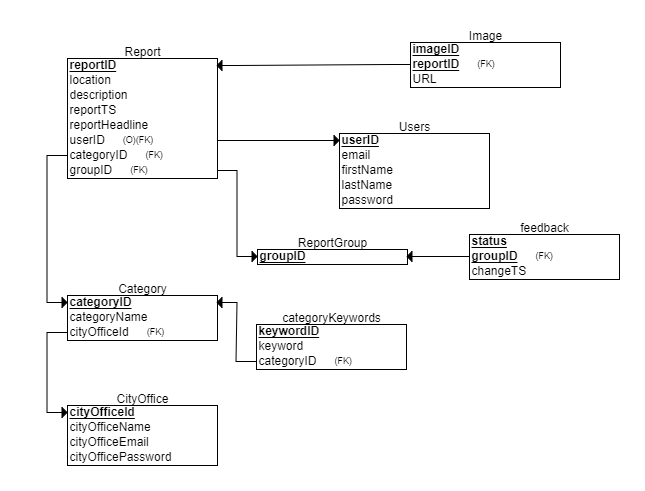
\includegraphics[width=\textwidth]{slike/relacijski.png} %veličina u odnosu na širinu linije
				\caption{Relacijski dijagram baze podataka}
				\label{fig:DijagramBazePodataka} %label mora biti drugaciji za svaku sliku
			\end{figure}
			
			\eject
			
			
		\section{Dijagram razreda}
		
			Na slikama \ref{fig:kontroler}, \ref{fig:dao}, \ref{fig:repo}, \ref{fig:service} su prikazani razredi koji pripadaju backend dijelu aplikacije. Razredi su arhitekturom podijeljeni na kontrolere, repozitorije i servise. Također postoje Domain i DTO (Data Transfer Object) modeli. Svi dijagrami su podložni promjenama, s obzirom na to da je aplikacija još uvijek u fazi razvoja.
		
			Slika \ref{fig:kontroler} prikazuje klase koje imaju ulogu kontrolera, tj. u kodu imaju anotaciju @RestController. Te klase definiraju endpointove i koriste se za dohvat i manipuliranje podacima iz baze podataka. ClientForwardController je kontroler koji povezuje Spring server React aplikacijom. Klase sa @RestController anotacijom koriste instance servisa. Servisi su klase koje imaju @Service anotaciju. Servisi implementiraju metode za upis (npr. createUser(Users);, createCitiyOffice(cityOffice), itd.), brisanje, dohvat i izmjenu podataka u bazi. Klasa ServerApplication je glavna klasa koja pokreće aplikaciju, a ServerApplicationTest služi za testiranje funkcionalnosti aplikacije, ali još nema implementiranu nikakvu funkcionalnost.
		
			\begin{figure}[H]
				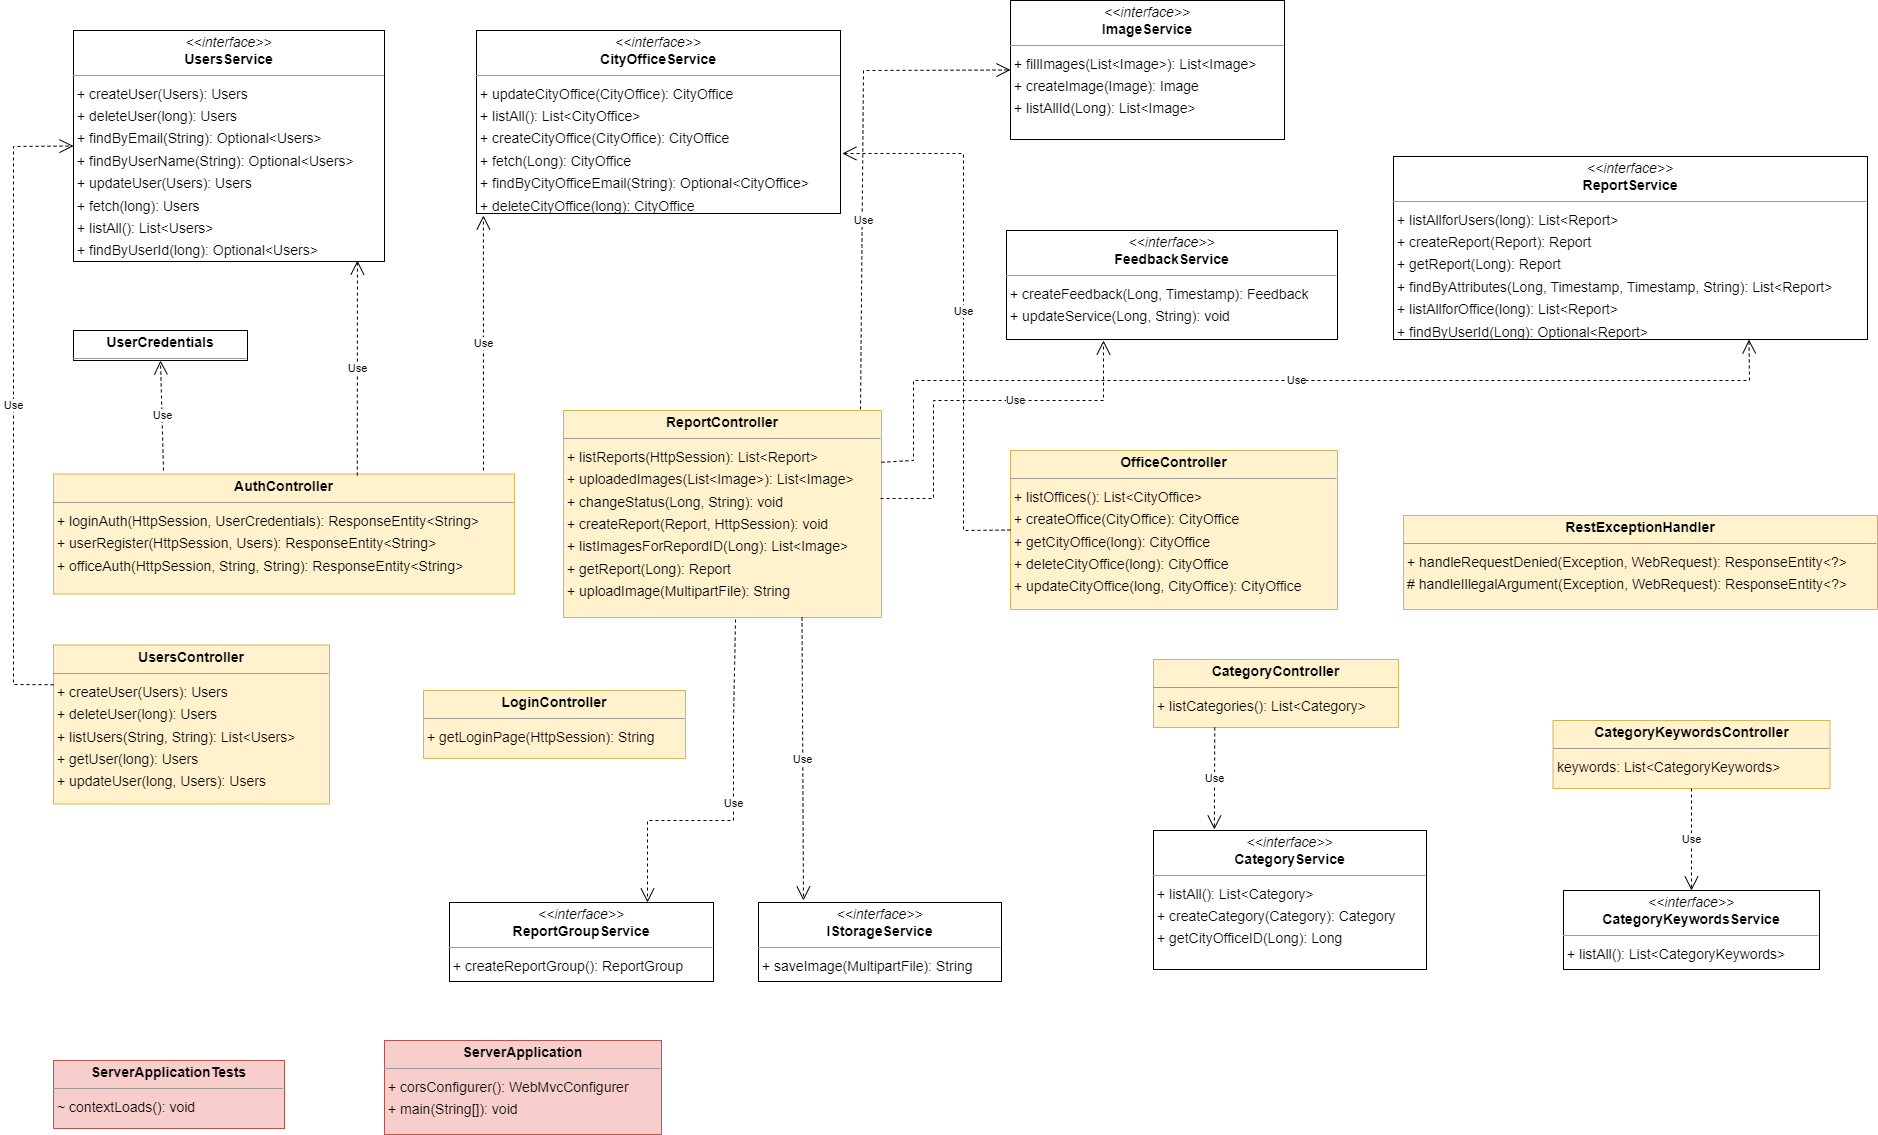
\includegraphics[width=\textwidth]{slike/controller.png} %veličina u odnosu na širinu linije
				\caption{Kontroleri na backendu}
				\label{fig:kontroler} %label mora biti drugaciji za svaku sliku
			\end{figure}
			
			\eject
			
			Slika \ref{fig:dao} prikazuje sučelja koja nasljeđuju sučelje JpaRepository. Sučelje JpaRepository definira razne CRUD (create, read, update, delete) metode za rad nad entitetima u bazi. Definirane metode izvršavaju razne vrste upite nad bazom podataka.
			
			\begin{figure}[H]
				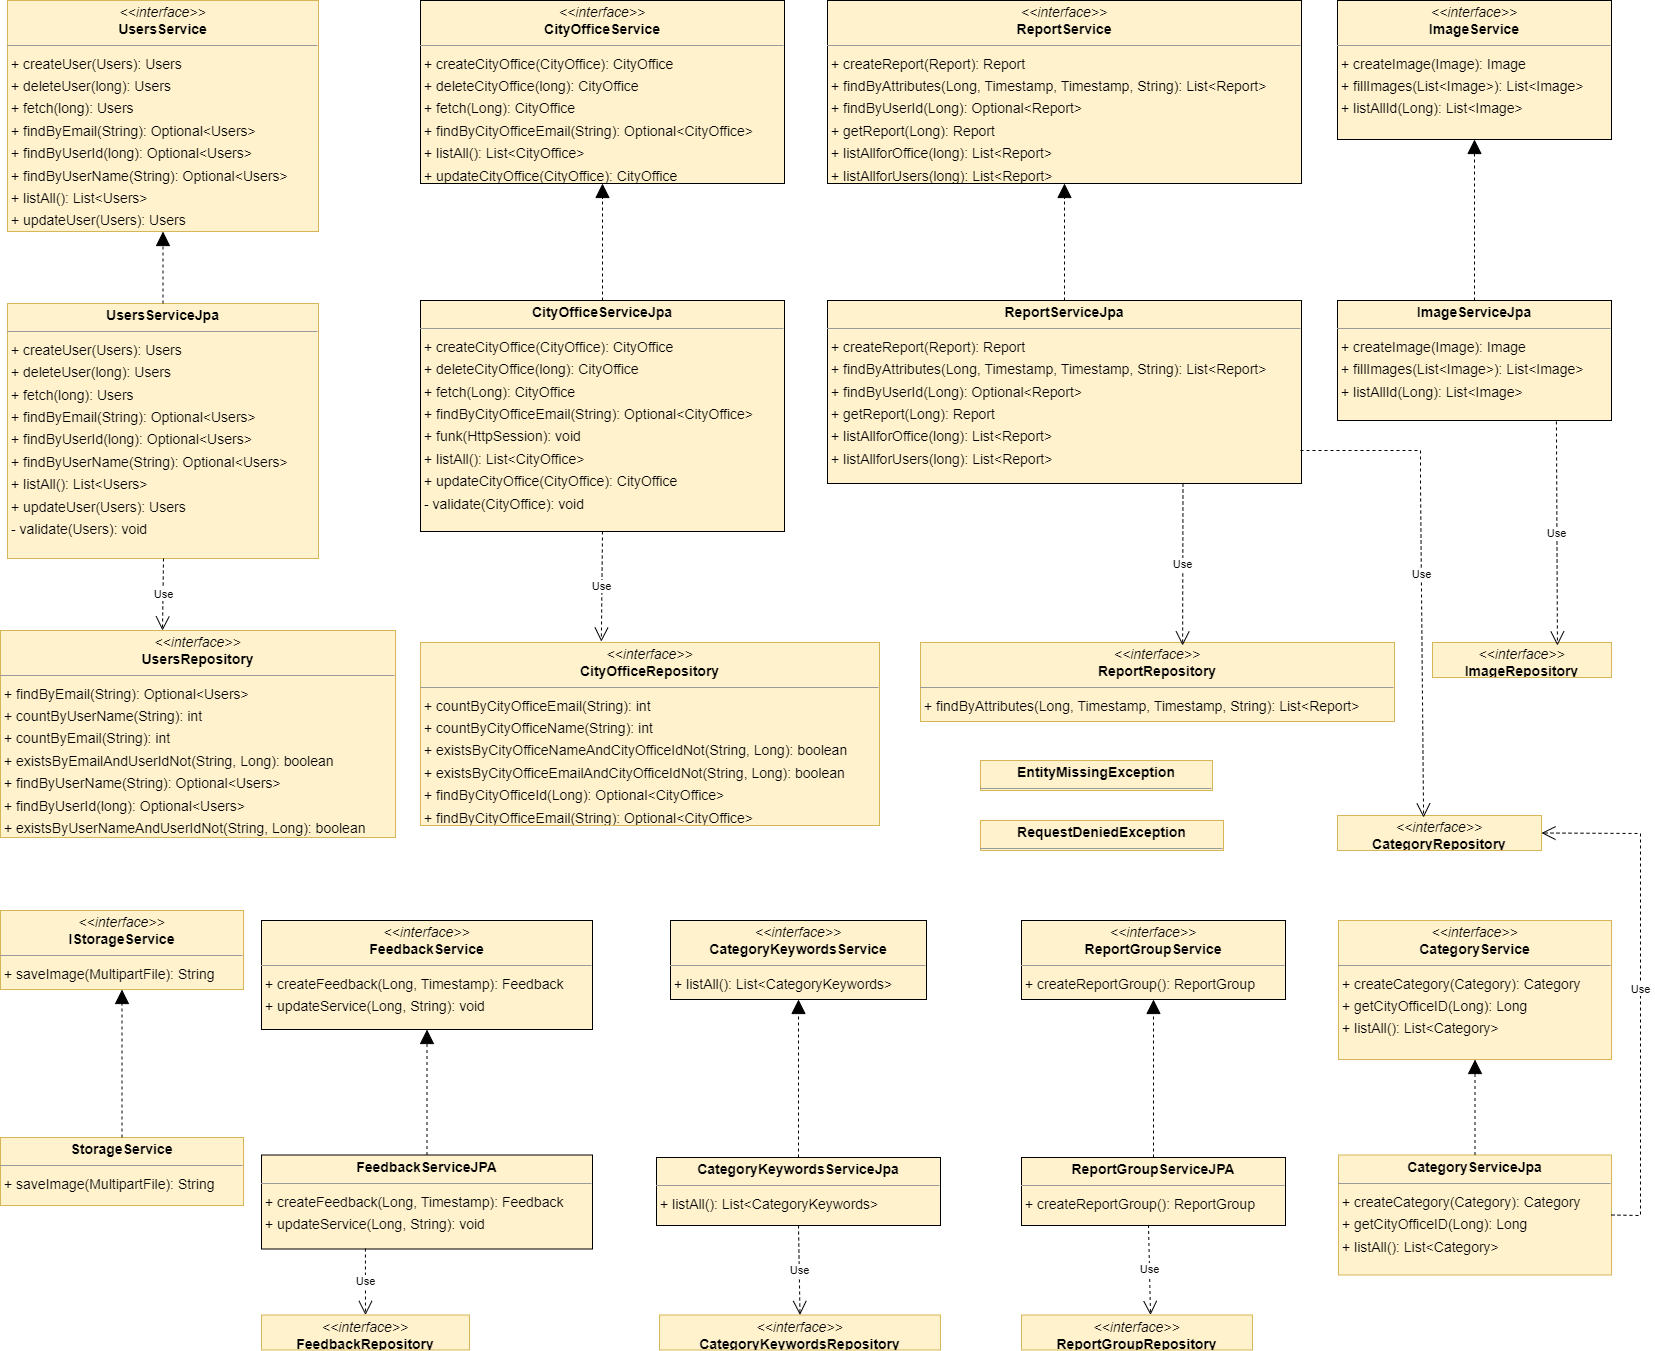
\includegraphics[width=\textwidth]{slike/dao.png} %veličina u odnosu na širinu linije
				\caption{Data Access Objects}
				\label{fig:dao} %label mora biti drugaciji za svaku sliku
			\end{figure}
			
			\eject
			
			Slika \ref{fig:repo} prikazuje klase u paketu repo koje reprezentiraju entitete u bazi podataka te njihove međusobne veze. Ove klase definiraju tipove atributa pojedinih entiteta, ograničenja nad atributima i primarne i strane ključeve. Svaka klasa ima implementirane metode get() i set() za svaki od atributa, kao i odgovarajuće konstruktore. Klasa FeedbackID služi kao pomoćna klasa za definiranje primarnog ključa feedback. Korisnici (Users) stvaraju prijave (Report), a gradski uredi (CityOffice) upravljaju prijavama i prilikom promjena automatski zapisuje nove povratne informacije (Feedback) u bazu podataka za tu grupu prijava.
			
			\begin{figure}[H]
				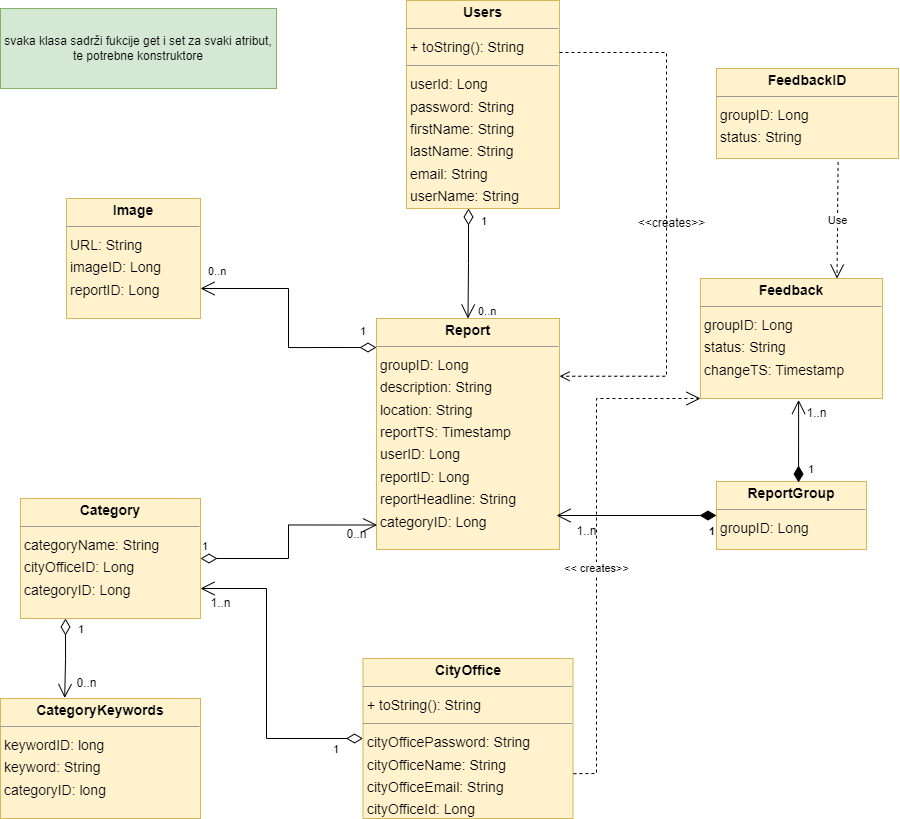
\includegraphics[width=\textwidth]{slike/repo.png} %veličina u odnosu na širinu linije
				\caption{Modeli}
				\label{fig:repo} %label mora biti drugaciji za svaku sliku
			\end{figure}
			
			\eject
			
			Slika \ref{fig:service} prikazuje klase servisa koje definiraju metode za CRUD operacije nad bazom podataka. EntityMissingException i RequestDeniedException su pomoćne klase za baratanje pogreškama. Klase servisa koriste instance Repository klasa iz slike 2. za poziv metoda definiranih u sklopu sučelja Repository odnosno JpaRepository.
			
			\begin{figure}[H]
				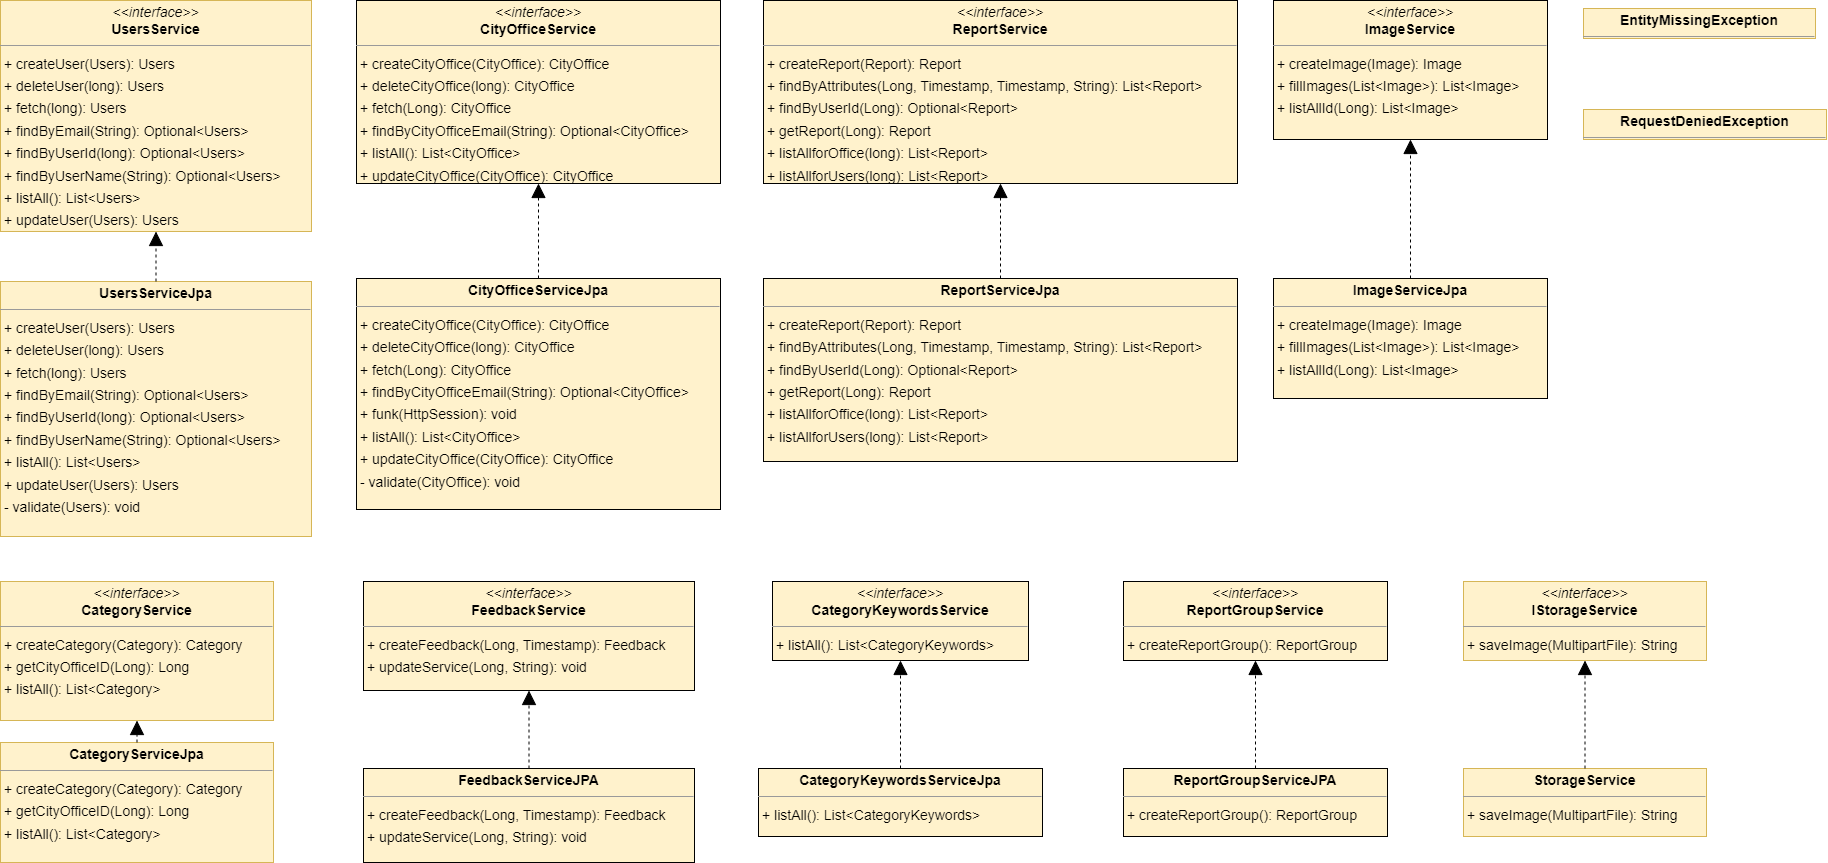
\includegraphics[width=\textwidth]{slike/service.png} %veličina u odnosu na širinu linije
				\caption{Servisi}
				\label{fig:service} %label mora biti drugaciji za svaku sliku
			\end{figure}
			
			\eject
			
			
			\section{Dijagram stanja}
			
			Dijagram stanja je vrsta UML dijagrama koja prikazuje stanja objekta i prijelaze između stanja. Prijelazi se aktiviraju određenim događajima i opcionalno dodatnim uvjetima. 
			
			Slika \ref{fig:dijagramStanja} prikazuje dijagram stanja za korisnika koji može, ali i ne mora biti prijavljen u sustav. 
			
			Korisniku je na početku prikazana glavna stranica na kojoj je karta sa prikazanim aktivnim prijavama u sustavu. Zaglavlje stranice sadrži gumbove za podnošenje nove prijave oštećenja ("Prijava štete"), prikaz statistike prijava ("Statistika"). Također, zaglavlje sadrži gumb sa e-mailom korisnika koji služi za upravljanje korisničkim računom ako je korisnik prijavljen u sustav. Ako korisnik nije prijavljen, zaglavlje sadrži gumbove za prijavu ("Log in") i registraciju ("Register") u  sustav. S obzirom da je zaglavlje isto na svim dijelovima aplikacije, korisnik ima pristup ovim opcijama bilo gdje u aplikaciji.
			
			Na glavnoj stranici korisnik može odabrati filtar prijava. Pomoću tog filtra korisnik može filtrirati aktivne prijave u sustavu koje će se prikazati na karti na početnoj stranici. Odabirom neke od prikazanih prijava na karti korisniku se otvara stranica odabrane prijave.
			
			Kod pregleda statistike prijava korisnik mora ispuniti obrazac filtra. Nakon potvrde obrasca korisniku se prikazuje statistika prijava koje su odabrane pomoću filtra. 
			
			Prilikom prijave novog oštećenja korisnik ispunjava obrazac prijave. Kada je u obrazac upisan opis oštećenja, sustav korisniku predlaže kategoriju oštećenja. Kada korisnik podnese prijavu, sustav provjerava ako već postoji slična prijava. Ako postoji, sustav nudi korisniku nadovezivanje njegove prijave na postojeću. Korisnik to može prihvatiti, ali može i poslati nepovezanu prijavu. Nakon konačnog podnošenja prijave sustav korisniku prikazuje jedinstveni kod prijave. Korisnik se vraća na početnu stranicu kada potvrdi zaprimljeni kod prijave.
			
			Ako je korisnik prijavljen može pregledati podatke o svojem korisničkom računu. Prilikom pregleda korisničkog računa može dodatno pregledavati vlastite prijave. Kada želi pregledati neku od prijava, korisniku se prikazuje stranica te prijave, isto kao i kod pregleda svih prijava na početnoj stranici. Korisnik također može mijenjati podatke o svojem korisničkom računu. Kod potvrde se izmjene spremaju, ako je do njih došlo. Također, korisnik kod pregleda računa može izbrisati svoj račun čime on postaje neprijavljen i neregistriran.
			
			\begin{figure}[H]
				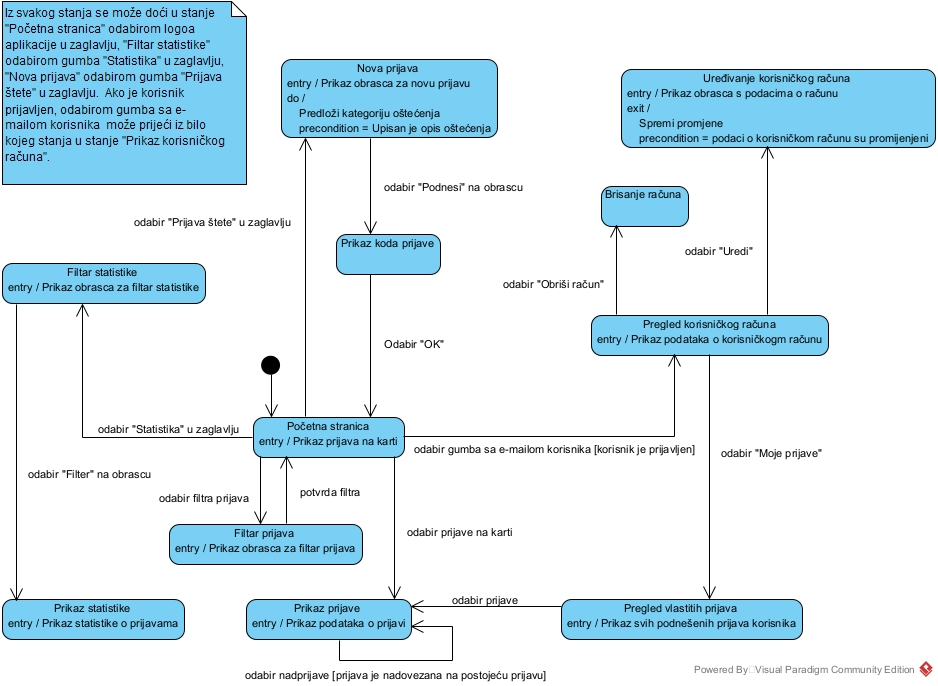
\includegraphics[width=\textwidth]{slike/dijagramStanja.jpg} %veličina u odnosu na širinu linije
				\caption{Dijagram stanja}
				\label{fig:dijagramStanja} %label mora biti drugaciji za svaku sliku
			\end{figure}
			
			\eject 
			
			\section{Dijagram aktivnosti}
			
			Dijagram aktivnosti je ponašajni UML dijagram koji modelira ponašanje sustava nizom akcija koje zajedno čine aktivnost. Dijagram aktivnosti se primjenjuje za modeliranje upravljačkog i podatkovnog toka. Ovakav tip dijagrama nije preporučljiv za modeliranje sustava sa događajima poticanim ponašanjem. Kod dijagrama aktivnosti svaka akcija se izvršava nakon završavanja prethodne akcije. Općenito je u dijagramu aktivnosti naglasak na jednostavnosti prikaza.
			
			Na dijagramu \ref{fig:dijagramAktivnosti} prikazan je proces podnošenja prijave oštećenja i njezine obrade u gradskom uredu. 
			
			Korisnik odabire opciju "Prijava štete" te ispunjava podatke o oštećenju na dobivenom obrascu. Kada je unesen opis prijave, aplikacija pomoću ključnih riječi pokušava prepoznati kategoriju oštećenja koju predlaže korisniku. Korisnik može prihvatiti predloženu kategoriju ili ručno odabrati drugu. Nakon što korisnik podnese prijavu, sustav provjerava ako već postoji slična prijava spremljena u bazi podataka. Ako postoji, sustav predlaže korisniku nadovezivanje njegove prijave na postojeću. Korisnik može, ali ne mora prihvatiti prijedlog i nakon toga potvrditi slanje prijave.
			
			Nakon što je prijava podnesena i spremljena u bazu podataka, djelatnik gradskog ureda može obraditi tu prijavu. Ako smatra da je prijava nevaljala, djelatnik ju odbacuje. Ako je prijava podnesena krivom uredu, korisnik prijavu može proslijediti drugom uredu. Ako je prijava valjana, djelatnik tu prijavu šalje gradskoj službi za sanaciju oštećenja. U svakom od navedenih slučaja promjena u prijavi se sprema u bazu podataka i obavještava se korisnika koji je podnio prijavu, ako je korisnik registriran u sustavu. Na kraju, kada gradska služba sanira oštećenje iz valjane prijave, ta se promjena također evidentira u bazi podataka i obavještava se korisnik kao i u ostalim slučajevima. 
			
			\begin{figure}[H]
				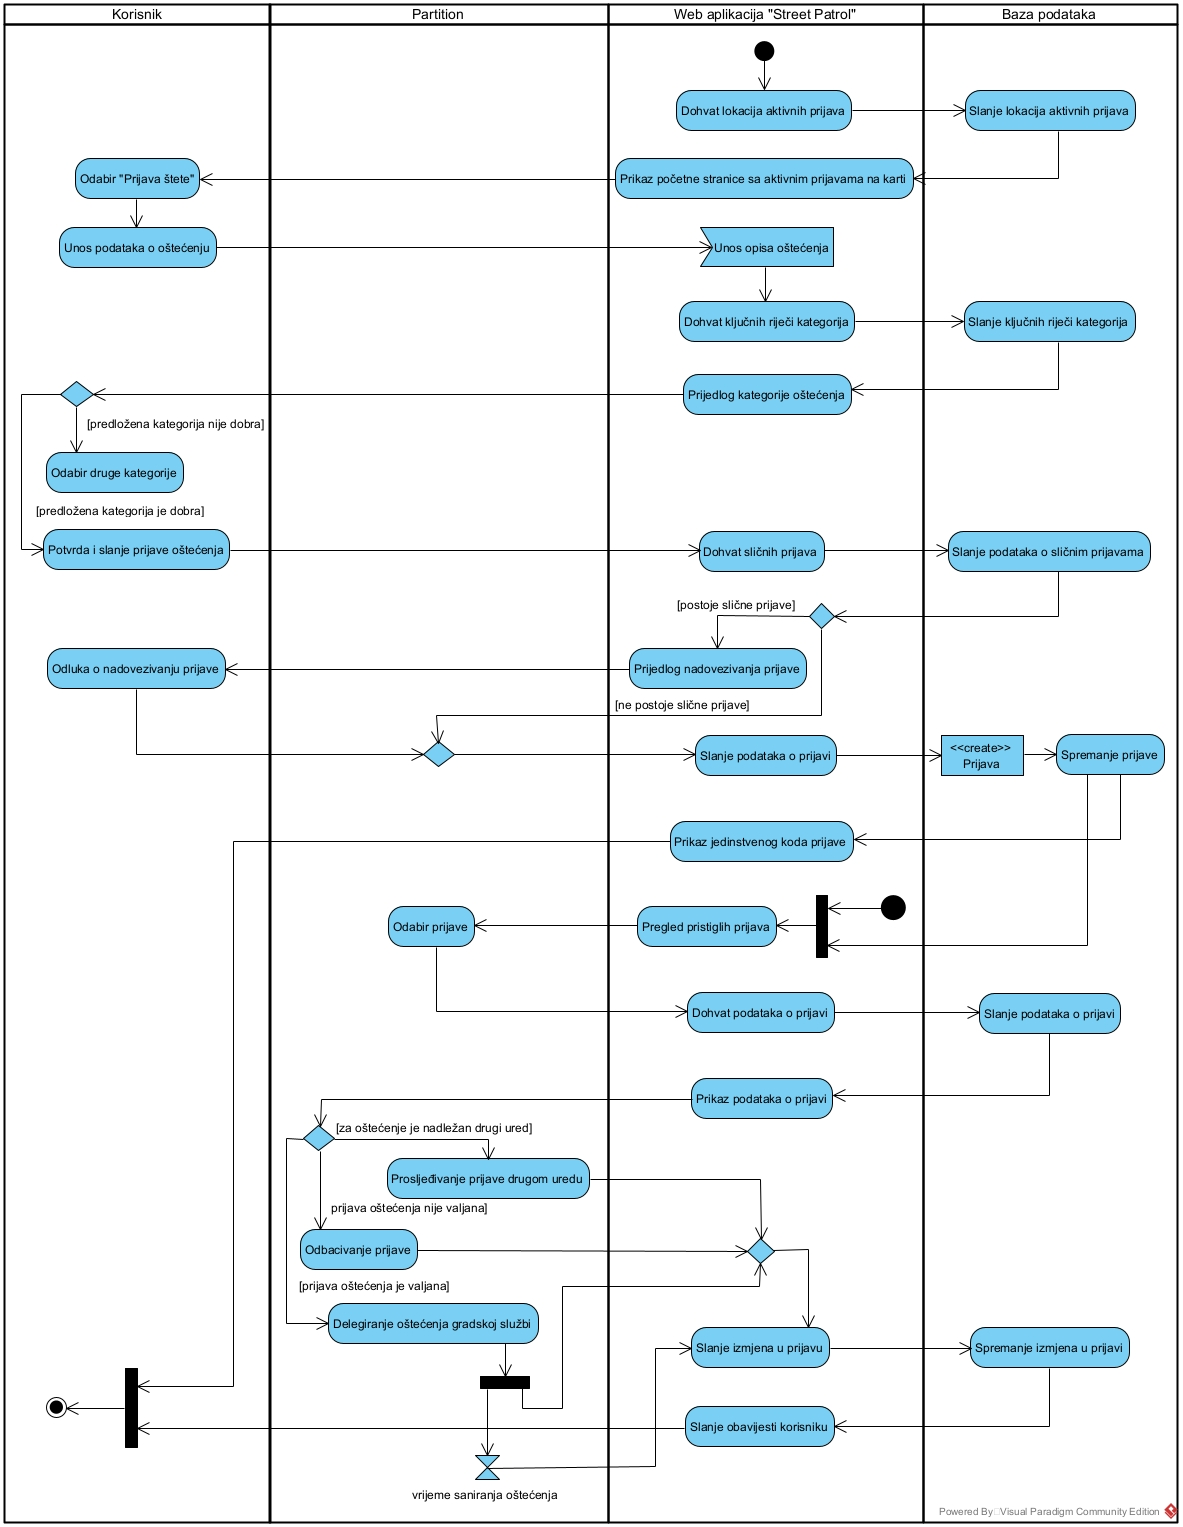
\includegraphics[width=\textwidth]{slike/dijagramAktivnosti.jpg} %veličina u odnosu na širinu linije
				\caption{Dijagram aktivnosti}
				\label{fig:dijagramAktivnosti} %label mora biti drugaciji za svaku sliku
			\end{figure}
			
			\eject
			
			\section{Dijagram komponenti}
	
			Dijagram komponenti je strukturni statički UML dijagram koji je dio specifikacije arhitekture programske potpore. Njime se vizualizira organizacija i međuovisnost između implementacijskih komponenata i odnos same programske okoline prema okolini. Ovakav tip dijagrama je pogodan kod komponentno-usmjerenog modela razvoja programske potpore i uslužno-orijentirane arhitekture. Osnovni elementi dijagrama komponenti su komponente, sučelja i poveznice.
			
			Na dijagramu \ref{fig:dijagramKomponenti} je prikazana organizacija i međuovisnost komponenata i sučelja u sustavu za prijavu oštećenja na javnim površinama. Dijagram se sastoji od komponente \textit{Web preglednik}, \textit{PostgreSQL baza podataka} i \textit{Web aplikacija}. \textit{Web aplikacija} ima dvije pod-komponente: \textit{React frontend} i \textit{Spring Boot backend}. 
			
			Pomoću \textit{Web preglednik} komponente se šalju zahtjevi \textit{Wev aplikacija} komponenti za pojedinim stranicama preko sučelja za dohvat vizualnog sadržaja. \textit{React router} komponenta unutar \textit{React frontend} komponente na temelju URL-a dobivenog od komponente \textit{Web preglednik} donosi odluku koja će se datoteka dohvatiti, to jest koja će se stranica prikazati pomoću komponente \textit{React view}. Komponenta \textit{index.js} je početna komponenta koja služi kao korijen za sve ostale elemente za prikaz. \textit{ReactJS} je biblioteka za sami React. \textit{React view} komponenta po potrebi korisniku osvježava prikaz i preko REST API-ja razmjenjuje podatke sa \textit{Spring Boot backend} komponentom aplikacije u JSON formatu.
			
			\textit{Controller} komponenta unutar \textit{Spring Boot backend} komponente preko REST API-ja prima zahtjeve, šalje ih dalje na obradu i nakon obrade šalje odgovore na njih. \textit{Service} komponenta prima zahtjeve od \textit{Controller} komponente, obrađuje ih i po potrebi komunicira sa \textit{Repository} komponentom. \textit{Repository} komponenta komunicira sa \textit{JpaRepository} komponentom preko JPA sučelja, a \textit{JpaRepository} komponenta preko PSQL sučelja komunicira sa \textit{PostgreSQL baza podataka} komponentom koja služi za trajnu pohranu podataka. \textit{Controller}, \textit{Service} i \textit{Repository} komponente koriste \textit{DTO} komponentu koja služi za enkapsulaciju, organizaciju i razmjenu podataka između komponenti.
			
			\begin{figure}[H]
				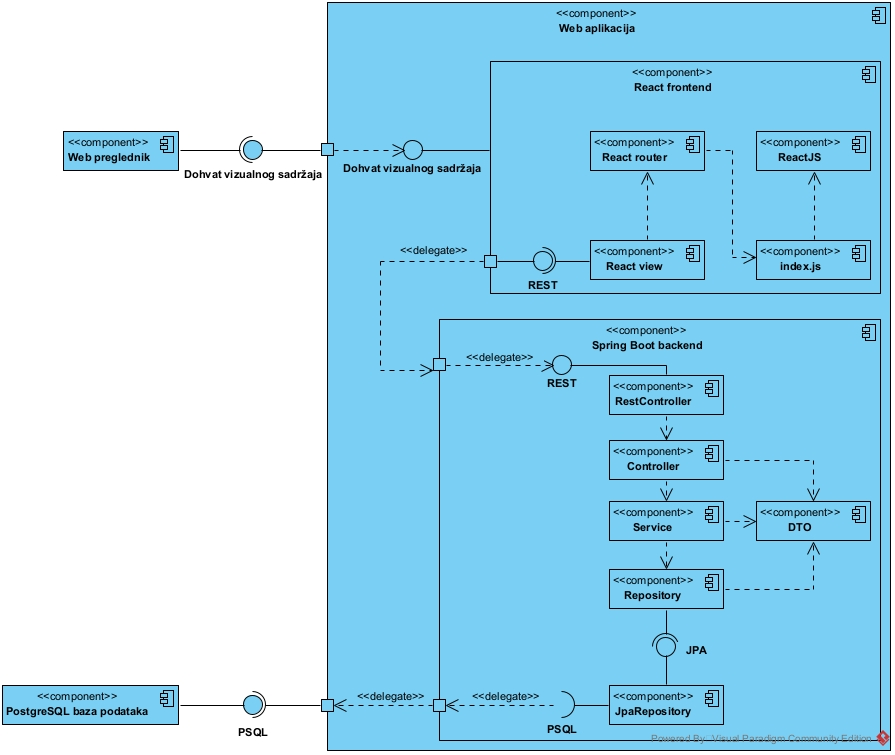
\includegraphics[width=\textwidth]{slike/dijagramKomponenti.jpg} %veličina u odnosu na širinu linije
				\caption{Dijagram komponenti}
				\label{fig:dijagramKomponenti} %label mora biti drugaciji za svaku sliku
			\end{figure}
			
			
			
			
			
			
			
			
			
			
			
			
			
	\chapter*{Popis literature}
		\addcontentsline{toc}{chapter}{Popis literature}		
		
		\begin{enumerate}
			
			\item GeeksForGeeks, Spring Boot Architecture, https://www.geeksforgeeks.org/spring-boot-architecture/
			
			\item  Programsko inženjerstvo, FER ZEMRIS, \url{http://www.fer.hr/predmet/proinz}
			
			\item Visual Paradigm, https://www.visual-paradigm.com/
			
			\item draw.io, https://app.diagrams.net/
			
			\item  The Unified Modeling Language, \url{https://www.uml-diagrams.org/}
			
			\item Baeldung, Spring Boot H2 database, https://www.baeldung.com/spring-boot-h2-database
			
		\end{enumerate}
		
		 
	
	
	\begingroup
	\renewcommand*\listfigurename{Indeks slika i dijagrama}
	%\renewcommand*\listtablename{Indeks tablica}
	%\let\clearpage\relax
	\listoffigures
	%\vspace{10mm}
	%\listoftables
	\endgroup
	\addcontentsline{toc}{chapter}{Indeks slika i dijagrama}


	
	\eject 
		
	\chapter*{Dodatak: Prikaz aktivnosti grupe}
		\addcontentsline{toc}{chapter}{Dodatak: Prikaz aktivnosti grupe}
		
		\section*{Dnevnik sastajanja}
		
		\textbf{\textit{Kontinuirano osvježavanje}}\\
		
		 \textit{U ovom dijelu potrebno je redovito osvježavati dnevnik sastajanja prema predlošku.}
		
		\begin{packed_enum}
			\item  sastanak
			
			\item[] \begin{packed_item}
				\item Datum: u ovom formatu: 23. listopada 2023.
				\item Prisustvovali: Petar Belošević, Vinko Brkić, Tomislav Grudić, Fran Meglić, Eno Peršić, Bruno Mikulan, Filip Vučenik
				\item Teme sastanka:
				\begin{packed_item}
					\item  napravljen git repozitorij
					\item  rasprava o zadatku - definirani ključni funkcijski i nefunkcijski zahtjevi, razmjena ideja oko aplikacije
					\item podjela poslova (pisanje opisa zadatka, izrada UML dijagrama, zapisivanje zahtjeva, raspodjela timova)
				\end{packed_item}
			\end{packed_item}
			
			\item  sastanak
			\item[] \begin{packed_item}
				\item Datum: u ovom formatu: 30. listopada 2023.
				\item Prisustvovali: Petar Belošević, Vinko Brkić, Tomislav Grudić, Fran Meglić, Eno Peršić, Bruno Mikulan, Filip Vučenik
				\item Teme sastanka:
				\begin{packed_item}
					\item  dizajn baze podataka
					\item  dizajn korisničkog sučelja aplikacije
					\item detaljnija rasprava o svojstvima aplikacije
				\end{packed_item}
			\end{packed_item}
			
			\item  sastanak
			\item[] \begin{packed_item}
				\item Datum: u ovom formatu: 6. studenoga 2023.
				\item Prisustvovali: Petar Belošević, Vinko Brkić, Tomislav Grudić, Fran Meglić, Eno Peršić, Bruno Mikulan, Filip Vučenik
				\item Teme sastanka:
				\begin{packed_item}
					\item  izvještaj svakog dijela tima o svojem napretku
					\item rad na dizajnu aplikacije
				\end{packed_item}
			\end{packed_item}
			
			\item  sastanak
			\item[] \begin{packed_item}
				\item Datum: u ovom formatu: 13. studenoga 2023.
				\item Prisustvovali: Petar Belošević, Vinko Brkić, Tomislav Grudić, Fran Meglić, Eno Peršić, Bruno Mikulan, Filip Vučenik
				\item Teme sastanka:
				\begin{packed_item}
					\item  izvještaj svakog dijela tima o svojem napretku
					\item korekcije na pojedinim dijelovima aplikacije
					\item rad na spajanju frontend i backend dijelova aplikacije
				\end{packed_item}
			\end{packed_item}
			%
			
		\end{packed_enum}
		
		\eject
		\section*{Tablica aktivnosti}
		
			\textbf{\textit{Kontinuirano osvježavanje}}\\
			
			 \textit{Napomena: Doprinose u aktivnostima treba navesti u satima po članovima grupe po aktivnosti.}

			\begin{longtblr}[
					label=none,
				]{
					vlines,hlines,
					width = \textwidth,
					colspec={X[7, l]X[1, c]X[1, c]X[1, c]X[1, c]X[1, c]X[1, c]X[1, c]}, 
					vline{1} = {1}{text=\clap{}},
					hline{1} = {1}{text=\clap{}},
					rowhead = 1,
				} 
			
				\SetCell[c=1]{c}{} & \SetCell[c=1]{c}{\rotatebox{90}{\textbf{Petar Belošević }}} & \SetCell[c=1]{c}{\rotatebox{90}{\textbf{Vinko Brkić }}} &	\SetCell[c=1]{c}{\rotatebox{90}{\textbf{Tomislav Grudić }}} & \SetCell[c=1]{c}{\rotatebox{90}{\textbf{Fran Meglić }}} &	\SetCell[c=1]{c}{\rotatebox{90}{\textbf{Bruno Mikulan }}} & \SetCell[c=1]{c}{\rotatebox{90}{\textbf{Eno Peršić }}} &	\SetCell[c=1]{c}{\rotatebox{90}{\textbf{Filip Vučenik }}} \\  
				Upravljanje projektom 		& 5 &  &  &  &  &  & \\ 
				Opis projektnog zadatka 	& 4 &  &  &  &  &  & 1 \\ 
				
				Funkcionalni zahtjevi       & 2 &  & 1 &  &  &  &  \\ 
				Opis pojedinih obrazaca 	& 2 &  &  &  &  &  &  \\ 
				Dijagram obrazaca 			& 2 &  &  &  & 2 &  &  \\ 
				Sekvencijski dijagrami 		& 2 & 1 &  & 1 &  &  &  \\ 
				Opis ostalih zahtjeva 		& 1 &  &  &  &  & 1 &  \\ 

				Arhitektura i dizajn sustava	 & 2 &  &  &  &  &  &  \\ 
				Baza podataka				& 1 &  & 2 &  &  &  &   \\ 
				Dijagram razreda 			&  &  &  &  &  &  &   \\ 
				Dijagram stanja				&  &  &  &  &  &  &  \\ 
				Dijagram aktivnosti 		&  &  &  &  &  &  &  \\ 
				Dijagram komponenti			&  &  &  &  &  &  &  \\ 
				Korištene tehnologije i alati 		&  &  &  &  &  &  &  \\ 
				Ispitivanje programskog rješenja 	&  &  &  &  &  &  &  \\ 
				Dijagram razmještaja			&  &  &  &  &  &  &  \\ 
				Upute za puštanje u pogon 		&  &  &  &  &  &  &  \\  
				Dnevnik sastajanja 			& 1 &  &  &  &  &  &  \\ 
				Zaključak i budući rad 		&  &  &  &  &  &  &  \\  
				Popis literature 			& 1 &  &  &  &  &  &  \\  
				&  &  &  &  &  &  &  \\ \hline 
				\textit{Dodatne stavke kako ste podijelili izradu aplikacije} 			&  &  &  &  &  &  &  \\ 
				\textit{rad na frontendu} 				&  & 6 &  &  & 6 & 6 &  \\  
				\textit{rad na backendu} 							&  &  & 6 & 6 &  &  & 6 \\
				\textit{izrada baze podataka} 		 			&  &  &  &  &  &  & \\  
				\textit{spajanje s bazom podataka} 							&  &  &  &  &  &  & \\ 
				\textit{usvajanje korištenih tehnologija} 							& 3 & 3 & 3 & 3 & 3 & 3 & 3 \\ 
			\end{longtblr}
					
					
		\eject
		\section*{Dijagrami pregleda promjena}
		
		\textbf{\textit{dio 2. revizije}}\\
		
		\textit{Prenijeti dijagram pregleda promjena nad datotekama projekta. Potrebno je na kraju projekta generirane grafove s gitlaba prenijeti u ovo poglavlje dokumentacije. Dijagrami za vlastiti projekt se mogu preuzeti s gitlab.com stranice, u izborniku Repository, pritiskom na stavku Contributors.}
		
	


\end{document} %naredbe i tekst nakon ove naredbe ne ulaze u izgrađen dokument 


